\documentclass[letterpaper,10pt,headsepline]{scrbook}
\usepackage[T1]{fontenc} 
\usepackage{natbib}
\usepackage{supertabular}
\usepackage{epsfig}
\usepackage{ifthen}
\usepackage{index}
\usepackage[backref,colorlinks]{hyperref}
\usepackage{listings}
\usepackage{verbatim}
\usepackage{hyphenat}
\usepackage{ragged2e}
\usepackage[acronym]{glossaries}
\usepackage{color}
\usepackage{tensor}
\usepackage{textcomp}
\usepackage{amssymb}
\usepackage{amsmath}
\usepackage{bm}

% Adaptive labelling.
\makeatletter
\newcommand{\iflabelexists}[3]{\@ifundefined{r@#1}{#3}{#2}}
\makeatother

% Table of contents
\setcounter{tocdepth}{5}

% Margins.
\setlength{\topmargin}{0mm}
\setlength{\textwidth}{160mm}
\setlength{\textheight}{210mm}
\setlength{\oddsidemargin}{0mm}
\setlength{\evensidemargin}{0mm}

% Useful commands.
% Names
\def\glc{{\normalfont \scshape Galacticus}}

% Physical constants.
\def\G{\mathrm{G}}
\def\clight{\mathrm{c}}
\def\d{\mathrm{d}}
\def\e{\mathrm{e}}

% Variable specifiers.
\def\void{\textcolor{red}{\textless void\textgreater}}
\def\logicalzero{\textcolor{red}{\textless logical\textgreater}}
\def\logicalone{\textcolor{red}{\textless logical(:)\textgreater}}
\def\logicaltwo{\textcolor{red}{\textless logical(:,:)\textgreater}}
\def\intzero{\textcolor{red}{\textless integer\textgreater}}
\def\intone{\textcolor{red}{\textless integer(:)\textgreater}}
\def\inttwo{\textcolor{red}{\textless integer(:,:)\textgreater}}
\def\intthree{\textcolor{red}{\textless integer(:,:,:)\textgreater}}
\def\doublezero{\textcolor{red}{\textless double\textgreater}}
\def\doubleone{\textcolor{red}{\textless double(:)\textgreater}}
\def\doubletwo{\textcolor{red}{\textless double(:,:)\textgreater}}
\def\doublethree{\textcolor{red}{\textless double(:,:,:)\textgreater}}
\def\enum{\textcolor{red}{\textless enumeration\textgreater}}
\def\argin{\textcolor{blue}{$\rightarrow$}}
\def\arginout{\textcolor{blue}{$\leftrightarrow$}}
\def\argout{\textcolor{blue}{$\leftarrow$}}

% Macros for linking to sections either through internal LaTeX label/ref or externally through hyperdef/hyperref.
%% Link to a class by class name.
\newcommand{\refClass}[1]{\ifthenelse{\equal{\docname}{Development}}{{\normalfont \ttfamily #1} (see \S\ref{class:#1})}{\href{https://github.com/galacticusorg/galacticus/releases/download/bleeding-edge/Galacticus_Development.pdf\#class.#1}{\normalfont \ttfamily #1}}}
%% Link to a physics description by class name.
\newcommand{\refPhysics}[1]{\ifthenelse{\equal{\docname}{Physics}}{{\normalfont \ttfamily #1} (see \S\ref{phys:#1})}{\href{https://github.com/galacticusorg/galacticus/releases/download/bleeding-edge/Galacticus_Physics.pdf\#physics.#1}{\normalfont \ttfamily #1}}}

%  These Macros are taken from the AAS TeX macro package version 5.2
%  and are compatible with the macros in the A&A document class
%  version 7.0

% Abbreviations for journals.  The object here is to provide authors
% with convenient shorthands for the most "popular" (often-cited)
% journals; the author can use these markup tags without being concerned
% about the exact form of the journal abbreviation, or its formatting.
% It is up to the keeper of the macros to make sure the macros expand
% to the proper text.  If macro package writers agree to all use the
% same TeX command name, authors only have to remember one thing, and
% the style file will take care of editorial preferences.  This also
% applies when a single journal decides to revamp its abbreviating
% scheme, as happened with the ApJ (Abt 1991).

\def\refjnl#1{{\normalfont \rmfamily#1}}

\def\aj{\refjnl{AJ}}                   % Astronomical Journal
\def\actaa{\refjnl{Acta Astron.}}      % Acta Astronomica
\def\araa{\refjnl{ARA\&A}}             % Annual Review of Astron and Astrophys
\def\apj{\refjnl{ApJ}}                 % Astrophysical Journal
\def\apjl{\refjnl{ApJ}}                % Astrophysical Journal, Letters
\def\apjs{\refjnl{ApJS}}               % Astrophysical Journal, Supplement
\def\ao{\refjnl{Appl.~Opt.}}           % Applied Optics
\def\apss{\refjnl{Ap\&SS}}             % Astrophysics and Space Science
\def\aap{\refjnl{A\&A}}                % Astronomy and Astrophysics
\def\aapr{\refjnl{A\&A~Rev.}}          % Astronomy and Astrophysics Reviews
\def\aaps{\refjnl{A\&AS}}              % Astronomy and Astrophysics, Supplement
\def\azh{\refjnl{AZh}}                 % Astronomicheskii Zhurnal
\def\baas{\refjnl{BAAS}}               % Bulletin of the AAS
\def\bac{\refjnl{Bull. astr. Inst. Czechosl.}}
                % Bulletin of the Astronomical Institutes of Czechoslovakia
\def\caa{\refjnl{Chinese Astron. Astrophys.}}
                % Chinese Astronomy and Astrophysics
\def\cjaa{\refjnl{Chinese J. Astron. Astrophys.}}
                % Chinese Journal of Astronomy and Astrophysics
\def\icarus{\refjnl{Icarus}}           % Icarus
\def\jcap{\refjnl{J. Cosmology Astropart. Phys.}}
                % Journal of Cosmology and Astroparticle Physics
\def\jrasc{\refjnl{JRASC}}             % Journal of the RAS of Canada
\def\memras{\refjnl{MmRAS}}            % Memoirs of the RAS
\def\mnras{\refjnl{MNRAS}}             % Monthly Notices of the RAS
\def\na{\refjnl{New A}}                % New Astronomy
\def\nar{\refjnl{New A Rev.}}          % New Astronomy Review
\def\pra{\refjnl{Phys.~Rev.~A}}        % Physical Review A: General Physics
\def\prb{\refjnl{Phys.~Rev.~B}}        % Physical Review B: Solid State
\def\prc{\refjnl{Phys.~Rev.~C}}        % Physical Review C
\def\prd{\refjnl{Phys.~Rev.~D}}        % Physical Review D
\def\pre{\refjnl{Phys.~Rev.~E}}        % Physical Review E
\def\prl{\refjnl{Phys.~Rev.~Lett.}}    % Physical Review Letters
\def\pasa{\refjnl{PASA}}               % Publications of the Astron. Soc. of Australia
\def\pasp{\refjnl{PASP}}               % Publications of the ASP
\def\pasj{\refjnl{PASJ}}               % Publications of the ASJ
\def\rmxaa{\refjnl{Rev. Mexicana Astron. Astrofis.}}%
                % Revista Mexicana de Astronomia y Astrofisica
\def\qjras{\refjnl{QJRAS}}             % Quarterly Journal of the RAS
\def\skytel{\refjnl{S\&T}}             % Sky and Telescope
\def\solphys{\refjnl{Sol.~Phys.}}      % Solar Physics
\def\sovast{\refjnl{Soviet~Ast.}}      % Soviet Astronomy
\def\ssr{\refjnl{Space~Sci.~Rev.}}     % Space Science Reviews
\def\zap{\refjnl{ZAp}}                 % Zeitschrift fuer Astrophysik
\def\nat{\refjnl{Nature}}              % Nature
\def\iaucirc{\refjnl{IAU~Circ.}}       % IAU Cirulars
\def\aplett{\refjnl{Astrophys.~Lett.}} % Astrophysics Letters
\def\apspr{\refjnl{Astrophys.~Space~Phys.~Res.}}
                % Astrophysics Space Physics Research
\def\bain{\refjnl{Bull.~Astron.~Inst.~Netherlands}}
                % Bulletin Astronomical Institute of the Netherlands
\def\fcp{\refjnl{Fund.~Cosmic~Phys.}}  % Fundamental Cosmic Physics
\def\gca{\refjnl{Geochim.~Cosmochim.~Acta}}   % Geochimica Cosmochimica Acta
\def\grl{\refjnl{Geophys.~Res.~Lett.}} % Geophysics Research Letters
\def\jcp{\refjnl{J.~Chem.~Phys.}}      % Journal of Chemical Physics
\def\jgr{\refjnl{J.~Geophys.~Res.}}    % Journal of Geophysics Research
\def\jqsrt{\refjnl{J.~Quant.~Spec.~Radiat.~Transf.}}
                % Journal of Quantitiative Spectroscopy and Radiative Transfer
\def\memsai{\refjnl{Mem.~Soc.~Astron.~Italiana}}
                % Mem. Societa Astronomica Italiana
\def\nphysa{\refjnl{Nucl.~Phys.~A}}   % Nuclear Physics A
\def\physrep{\refjnl{Phys.~Rep.}}   % Physics Reports
\def\physscr{\refjnl{Phys.~Scr}}   % Physica Scripta
\def\planss{\refjnl{Planet.~Space~Sci.}}   % Planetary Space Science
\def\procspie{\refjnl{Proc.~SPIE}}   % Proceedings of the SPIE

\let\astap=\aap
\let\apjlett=\apjl
\let\apjsupp=\apjs
\let\applopt=\ao


% Define which document we are building.
\newcommand{\docname}{Physics}

% Build glossary and index.
\makeglossaries
\glstoctrue
\makeindex

% Acronyms.
\newacronym{cdm}{CDM}{cold dark matter}
\newacronym{cmb}{CMB}{cosmic microwave background}
\newacronym{igm}{IGM}{intergalactic medium}
\newacronym{imf}{IMF}{initial mass function}
\newacronym{isco}{ISCO}{innermost stable circular orbit}
\newacronym{ism}{ISM}{interstellar medium}
\newacronym{ode}{ODE}{ordinary differential equation}
\newacronym{nfw}{NFW}{Navarro-Frenk-White (dark matter halo profile)}
\newacronym{sed}{SED}{spectral energy distribution}
\newacronym{sne}{SNe}{supernovae}
\newglossaryentry{adaf}{type=\acronymtype, name={ADAF}, description=\glslink{adafg}{advection-dominated accretion flow}, first={advection-dominated accretion flow (ADAF)}, see=[Glossary:]{adafg}}
\newglossaryentry{pah}{type=\acronymtype, name={PAH}, description=\glslink{pahg}{polycyclic aromatic hydrocarbon}, first={polycyclic aromatic hydrocarbon (PAH)}, see=[Glossary:]{pahg}, firstplural={polycyclic aromatic hydrocarbons (PAH)}, see=[Glossary:]{pahg}}
\newglossaryentry{dsl}{type=\acronymtype, name={DSL}, description=\glslink{dslg}{domain-specific language}, first={domain specific language (DSL)}, see=[Glossary:]{dslg}, firstplural={domain-specific languages (DSLs)}, see=[Glossary:]{dslg}}
\newacronym{sdss}{SDSS}{Sloan Digitial Sky Survey}
\newglossaryentry{ahf}{type=\acronymtype, name={AHF}, description=\glslink{ahfg}{Amiga's Halo Finder}, first={Amiga's Halo Finder (AHF)}, see=[Glossary:]{ahfg}}
\newacronym{mcmc}{MCMC}{Markov Chain Monte Carlo}
\newglossaryentry{sam}{type=\acronymtype, name={SAM}, description=\glslink{samg}{semi-analytic model}, first={semi-analytic model (SAM)}, see=[Glossary:]{samg}, firstplural={semi-analytic models (SAMs)}, see=[Glossary:]{samg}}
\newglossaryentry{bie}{type=\acronymtype, name={BIE}, description=\glslink{bieg}{semi-analytic model}, first={Bayesian inference engine (BIE)}, see=[Glossary:]{bieg}, firstplural={Bayesian inference engines (BIEs)}, see=[Glossary:]{bieg}}
\newglossaryentry{hod}{type=\acronymtype, name={HOD}, description=\glslink{hodg}{halo occupation distribution}, first={halo occupation distribution (HOD)}, see=[Glossary:]{hodg}, firstplural={halo occupation distributions (HODs)}, see=[Glossary:]{hodg}}
\newglossaryentry{mpi}{type=\acronymtype, name={MPI}, description=\glslink{mpig}{message passing interface}, first={message passing interface (MPI)}, see=[Glossary:]{mpig}, firstplural={message passing interfaces (MPIs)}, see=[Glossary:]{mpig}}
\newglossaryentry{pbs}{type=\acronymtype, name={PBS}, description=\glslink{pbsg}{portable batch system}, first={portable batch system (PBS)}, see=[Glossary:]{pbsg}, firstplural={portable batch systems (PBSs)}, see=[Glossary:]{pbsg}}

% Glossary entries.
\newglossaryentry{FFTLog}{name={FFTLog}, description={\href{http://casa.colorado.edu/~ajsh/FFTLog/}{FFTLog} is a code to compute fast Fourier transforms of discrete periodic sequences of logarithmically spaced data}}

\newglossaryentry{component}{name={component}, description={An individual physical system within a \gls{node}, such as a dark matter halo, a galactic disk or a supermassive black hole}}

\newglossaryentry{forest}{name={forest}, description={A collection of merger trees that are linked together by virtue of nodes which jump between trees}}

\newglossaryentry{node}{name={node}, description={A single point in a merger tree, consisting of a dark matter halo and associated baryons}}

\newglossaryentry{mergee}{name={mergee}, description={For a given node in a merger tree, the set of mergee nodes consists of all nodes which will undergo a galaxy merger with the node at some point in the future}}

\newglossaryentry{primary progenitor}{name={primary progenitor}, description={The progenitor of a given \gls{node} which is regarding as the direct descendent of that \gls{node} (often, but not always, the most massive progenitor). Other progenitors are considered to merge into this primary progenitor}}

\newglossaryentry{parent}{name={parent}, description={In a merger tree, the parent node of any given node that exists at time $t_0$ is that node to which it is directly connected in the tree at time $t_1>t_0$}}

\newglossaryentry{Bernoulli distribution}{name={Bernoulli distribution}, description={A discrete probability distribution which takes value $1$ with success probability $p$ and value $0$ with failure probability $q = 1-p$. Read more on \href{http://en.wikipedia.org/wiki/Bernoulli_distribution}{Wikipedia}}}

\newglossaryentry{UUID}{name={UUID}, description={A \href{http://en.wikipedia.org/wiki/Universally_unique_identifier}{universally unique identifier}---this is a label which uniquely identifies some object (in this case, a \glc\ model)}}

\newglossaryentry{ABmagnitude}{name={AB magnitude}, description={An astronomical magnitude system in which the apparent magnitude is defined as $m=-2.5\log_{10}f-48.60$ for a flux density, $f$, measured in ergs per second per square centimeter per hertz}}

\newglossaryentry{forwardDescendent}{name={forward descendent}, description={The node with which the mass (or majority of the mass) of a node will become associated with at a later time. This type of descendent is usually relevant when considering how halos and galaxies evolve forward in time and should be distinguished from a \gls{backwardDescendent} which is relevant when building merger trees}}

\newglossaryentry{backwardDescendent}{name={backward descendent}, description={The \gls{primary progenitor} of a node. This type of descendent is usually relevant when building merger trees and should be distinguished from a \gls{forwardDescendent} which is relevant when considering how halos and galaxies evolve forward in time}}

\newglossaryentry{MD5hash}{name={MD5 hash}, description={The \href{http://en.wikipedia.org/wiki/MD5}{MD5 Message-Digest Algorithm} is a widely used cryptographic hash function that produces a 128-bit (16-byte) hash value. In \glc\ it is used to encode unique labels for modules which are incorporated into file names. \glc\ uses the \href{http://www.gnu.org/software/libc/}{\tt glibc} \href{http://en.wikipedia.org/wiki/Crypt_(Unix)}{\tt crypt()} function to compute MD5 hashes, but switches ``{\tt /}'' for ``{\tt @}'' in the hash (since ``{\tt /}'' is inconvenient for use in file names)}}

\newglossaryentry{LymanContinuum}{name={Lyman continuum}, description={The part of the electromagnetic spectrum which is capable of ionizing hydrogen, i.e. photons with wavelengths shorter than 91.1267~nanometres and with energy above 13.6~eV}}

\newglossaryentry{millenniumSimulation}{name={Millennium Simulation}, description={The \href{http://www.mpa-garching.mpg.de/galform/virgo/millennium/}{Millennium Simulation} is a high-resolution N-body simulation of structure formation in a cold dark matter universe.}}

\newglossaryentry{latinhypercube}{name={Latin hypercube}, description={A \href{http://en.wikipedia.org/wiki/Latin_hypercube_sampling}{Latin hypercube} is a construct for generating a sample of plausible collections of parameter values from a multidimensional distribution}}

\newglossaryentry{maximin}{name={maximin}, description={In \gls{latinhypercube} design, the ``maximin'' approach generates a large number of \glspl{latinhypercube} and selects the one which has the greatest minimum distance between all pairs of points in the hypercube}}

\newglossaryentry{mangle}{name={{\sc mangle}}, description={\href{http://space.mit.edu/~molly/mangle/}{\sc mangle} is a software package used for defining angular masks on the surface of a sphere. It is used primarily for defining the geometry of galaxy surveys}}

\newglossaryentry{adafg}{name={ADAF},
    description={An advection-dominated accretion flow (ADAF) is a particular solution for an accretion flow around a black hole, star or compact object in which energy liberated by viscous forces is stored within the accretion flow and advected inward to the central object (see \citealt{narayan_advection-dominated_1998})}}

\newglossaryentry{pahg}{name={PAH},
    description={\href{http://en.wikipedia.org/wiki/Polycyclic_aromatic_hydrocarbon}{Polycyclic aromatic hydrocarbons} (PAH) are large organic molecules consisting of fused aromatic rings}}

\newglossaryentry{dslg}{name={DSL},
    description={\href{http://en.wikipedia.org/wiki/Domain-specific_language}{Domain-specific languages} (DSL) are a type of programming language dedicated to a particular problem. In \glc\ a DSL is used to specify the structure of \glspl{component}}}

\newglossaryentry{samg}{name={SAM},
    description={Semi-analytic models (SAMs) are a type of galaxy formation model utilizing simple parameterizations of physical processes to follow the evolution of galaxies through a merging hierarchy of galaxies.}}

\newglossaryentry{ahfg}{name={AHF},
    description={\href{http://popia.ft.uam.es/AHF/files/AHF.pdf}{Amiga's Halo Finder} (AHF) is a software package which identifies dark matter halos in N-body simulations. Full details are given by \cite{gill_evolution_2004} and \cite{knollmann_ahf:_2009}}}

\newglossaryentry{hodg}{name={HOD},
    description={A halo occupation distribution (HOD) is a mathematical model describing the distribution of the number of galaxies (of some given physical properties) found in a dark matter halo of given mass.}}

\newglossaryentry{bieg}{name={BIE},
    description={The \href{http://www.astro.umass.edu/BIE/}{Bayesian Inference Engine} (BIE) is a software package designed to facilitate exploration of complexes parameter spaces using Bayesian techniques.}}

\newglossaryentry{mpig}{name={MPI},
    description={\href{http://en.wikipedia.org/wiki/Message_Passing_Interface}{Message Passing Interface} (MPI) is a standard for passing messages between processes on parallel computers.}}

\newglossaryentry{pbsg}{name={PBS},
    description={\href{http://en.wikipedia.org/wiki/Portable_Batch_System}{Portable Batch System} (PBS) is a job scheduler used on many compute cluster environments.}}


\begin{document}

\lstset{language=[95]Fortran}

\frontmatter

\pagestyle{empty}
\begin{center}
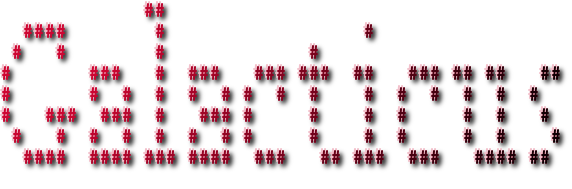
\includegraphics[width=125mm]{GalacticusLogo.png}\\

\Huge Physics Models \normalsize

\docname

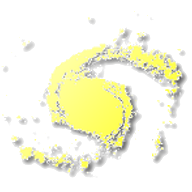
\includegraphics{New_Logo_Galaxy_192_Transparent.png}\\
A semi-analytic galaxy formation code.\\

\copyright\ 2009, 2010 2011, 2012, 2013, 2014, 2015, 2016, 2017, 2018, 2019, 2020, 2021, 2022, 2023, 2024, 2025 Andrew Benson
\end{center}

\tableofcontents

\mainmatter
\pagestyle{headings}

\chapter{Definitions and Conventions Used in \glc}

\glc\ adopts various definitions and conventions internally. These are explained below.

\section{Halo Masses and Dark Matter Mass}

Halo masses require some care in specifying exactly what mass they represent due to the way in which merger trees are typically created. For example, when merger trees are extracted from N-body simulations, those simulations frequently represent \emph{all} matter as collisionless. That is, the simulation contains a density $\Omega_\mathrm{M}=\Omega_\mathrm{DM}+\Omega_\mathrm{b}$ which is the sum of dark and baryonic matter densities, but all of this mass is represented as collisionless particles. Similarly, masses in merger trees built through Monte Carlo techniques typically represent all mass as collisionless.

The exact way in which masses within \glc\ are defined and used in specified in the following subsections.

\subsection{Masses in the Basic Component}

The {\normalfont \ttfamily basic} component (see \S\ref{sec:ComponentBasicProperties}) tracks the mass of each halo as defined in the merger tree. As such, it should be considered to be the mass which the halo would have if baryonic matter behaved just as dark matter. Note that these masses are inclusive of subhalos---that is, the mass of a host halo includes the mass of all of its subhalos.

\subsection{Dark Matter Profiles}

The dark matter profile functions (see \refPhysics{darkMatterProfileDMO}) return masses and densities etc. which are normalized to match the mass of the {\normalfont \ttfamily basic} component at the virial radius of the halo. As such, their returned values should be considered to represent the case where baryonic matter behaves as dark matter. This is a convention, and is useful for calculations of large scale structure for example.

\subsection{Galactic Structure Functions}

The various galactic structure functions assume that the masses/densities/etc. reported by the dark matter profile functions should be scaled by a factor $(\Omega_\mathrm{M}-\Omega_\mathrm{b})/\Omega_\mathrm{b}$ to leave only the dark matter part of the profile. Baryonic contributions to the mass/density/etc. will be provided by the components representing those mass distributions.

\subsection{Satellite Virial Orbits}

These functions (see \refPhysics{virialOrbit}) typically use the {\normalfont \ttfamily basic} component mass in determining parameters of an orbit, since they are typically calibrated to simulations of collisionless matter only.

\subsection{Satellite Merging Timescales}

These functions (see \refPhysics{satelliteMergingTimescales}) typically use the {\normalfont \ttfamily basic} component mass in determining parameters of an orbit, since they are typically calibrated to simulations of collisionless matter only.

\subsection{Dynamical Friction}

These functions (see \refPhysics{satelliteDynamicalFriction}) evaluate densities through the relevant galactic structure function, and so correctly account for the fraction of the {\normalfont \ttfamily basic} component mass which is in the form of dark matter.

\subsection{Galactic Structure Radius Solvers}

These functions \refPhysics{galacticStructureSolver}) determine the radii of galactic components (such as disk and spheroid), typically by iteratively seeking a solution in which their angular momenta and radii are consistent (assuming rotational support) with the net gravitational potential of the entire system (galaxy plus dark matter halo).

\section{Luminosity Units}

Galaxy luminosities are output in the \gls{ABmagnitude} system, such that a luminosity of $1$ corresponds to an object of $0^\mathrm{th}$ absolute magnitude in the \gls{ABmagnitude} system. This implies that the luminosities are in units of $4.4659\times 10^{13}$~W/Hz.

\section{Peculiar Velocities}\label{sec:GalacticusVelocityDefinitions}\hyperdef{sec}{peculiarVelocities}{}

Velocities in \glc\ are always \emph{physical} velocities. When reading merger tree properties (including velocities) from file it is often convenient to store velocities without the Hubble flow contribution, as ``peculiar velocities'', in the file---see \href{https://github.com/galacticusorg/galacticus/wiki/Merger-Tree-File-Format#forest-halos-group}{here} for how to specify whether or not  the velocities included in the file include the Hubble flow or not.

If peculiar velocities are stored it is important to use the same definition of peculiar velocity as is used by \glc. Defining $t$ to be physical time and $\mathbf{x}$ to be comoving position, \glc\ uses the conventional definition of peculiar velocity in a cosmological context, namely that it is the deviation of the physical velocity from the Hubble flow. Physical coordinates are given by $\mathbf{r} = a\mathbf{x}$, so the peculiar velocity is
\begin{equation}
\mathbf{v}_\mathrm{pec} \equiv {\mathrm{d} \mathbf{r} \over \mathrm{d} t} - H \mathbf{r} = a {\mathrm{d} \mathbf{x}\over\mathrm{d} t} = {\mathrm{d}\mathbf{x}\over\mathrm{d}\eta},
\end{equation}
where $\mathrm{d}\eta = \mathrm{d}t/a$ is conformal time. 

\section{Gravitational Potentials}\index{potential!gravitational}\index{gravitational potential}

Gravitational potentials are measured in velocity units (i.e. km$^2$/s$^2$), and the arbitrary constant offset is chosen such that the total gravitational potential in any halo at the virial radius is $\Phi(r_\mathrm{virial})=-V_\mathrm{virial}^2$. This choice is made for two reasons:
\begin{enumerate}
\item some mass distributions used have potentials which diverge as $r\rightarrow\infty$, so the usual choice of $\Phi(r) \rightarrow 0$ as $r \rightarrow \infty$ is not applicable;
\item this choice is consistent with the potential at the virial radius of the halo considered as a point mass as is used in Keplerian orbit calculations.
\end{enumerate}
Note that the choice of constant offset for the potential of any mass distribution or galactic component is irrelevant---the galactic structure function which computes potential will ensure that the potential is always offset to match the definition given above.

\section{Radius Specifiers}\label{sec:radiusSpecifiers}\index{radii!specifiers}\hyperdef{sec}{radiusSpecifiers}{}

Several \refClass{nodePropertyExtractorClass}s extract properties at one or more radii in a node. \glc\ provides a flexible way of specifying such radii as fractions of physical quantities such as the virial radius, disk half-mass radius, etc.

Each radius specifier should take the form:
\begin{verbatim}
  radiusType:componentType:massType:radius
\end{verbatim}
The elements of this colon-separated specifier determine the radius at which a property is computed, which components/mass types should be counted, and whether baryonic loading of the halo should be accounted for. The elements have the following meaning:
\begin{description}
 \item [{\normalfont \ttfamily radius}] the numerical value of the radius at which to compute the property (with units specified by the {\normalfont \ttfamily radiusType} element);
 \item [{\normalfont \ttfamily radiusType}] specifies the units of the {\normalfont \ttfamily radius} element---valid options are {\normalfont \ttfamily diskRadius}, {\normalfont \ttfamily hotHaloOuterRadius}, {\normalfont \ttfamily diskHalfMassRadius}, {\normalfont \ttfamily spheroidRadius}, {\normalfont \ttfamily spheroidHalfMassRadius}, {\normalfont \ttfamily darkMatterScaleRadius}, {\normalfont \ttfamily virialRadius}, just {\normalfont \ttfamily radius} (which implies radii are given in units of Mpc), {\normalfont \ttfamily galacticMassFraction\{\textless fraction\textgreater\}}, {\normalfont \ttfamily stellarMassFraction\{\textless fraction\textgreater\}}, or \newline {\normalfont \ttfamily galacticLightFraction\{\textless fraction\textgreater\}\{\textless luminosity\textgreater\}}, where the final three form specify a radius containing a fixed {\normalfont \ttfamily \textless fraction\textgreater} of the galactic or stellar mass, or light respectively (for the case of galactic light, {\normalfont \ttfamily \textless luminosity\textgreater} specifies the band, e.g. {\normalfont \ttfamily SDSS\_r:rest:z0.0000});
 \item [{\normalfont \ttfamily componentType}] specifies which components of the node should be counted---allowed values are {\normalfont \ttfamily all}, {\normalfont \ttfamily disk}, {\normalfont \ttfamily spheroid}, {\normalfont \ttfamily hotHalo}, {\normalfont \ttfamily darkHalo}, and {\normalfont \ttfamily blackHole};
 \item [{\normalfont \ttfamily massType}] specifies which types of mass should be counted---allowed values are {\normalfont \ttfamily all}, {\normalfont \ttfamily dark}, {\normalfont \ttfamily baryonic}, {\normalfont \ttfamily galactic}, {\normalfont \ttfamily gaseous}, {\normalfont \ttfamily stellar}, and {\normalfont \ttfamily blackHole}.
\end{description}

\section{Half-mode and quarter-mode masses}
For non-cold dark matter models with a matter power spectrum suppressed on small scales, a characteristic suppression scale can be defined by comparing the linear transfer function with that in the\gls{cdm} model. A popular definition is the half-mode (quarter-mode) mass, which corresponds to the wavenumber at which the transfer function is suppressed by a factor of two (four) relative to a \gls{cdm} transfer function.



\chapter{Node Components}\label{sec:Components}

In addition to the implementations described here, each component class has a ``{\normalfont \ttfamily null}'' implementation. Selecting this implementation---which has no properties and does not respond to any events---effectively switches off the relevant component class. Of course, this is safe only if none of the other active implementations expect to get or set properties of the component class (or if they rely on a sensible implementation of that class).

\section{(Supermassive) Black Hole}

\subsection{``Standard'' Implementation}

\subsubsection{Properties}

The standard black hole implementation defines the following properties:
\begin{description}
 \item [{\normalfont \ttfamily mass}] The mass of the black hole: $M_\bullet$ {\normalfont \ttfamily [blackHoleMass]}.
 \item [{\normalfont \ttfamily spin}] The spin of the black hole, $j_\bullet$ {\normalfont \ttfamily [blackHoleSpin]}.
 \item [{\normalfont \ttfamily radialPosition}] The radial position of the black hole: $r_\bullet$ {\normalfont \ttfamily [blackHoleRadialPosition]} 
\end{description}

\subsubsection{Initialization}

Black holes are not initialized, they are created (with a seed mass given by {\normalfont \ttfamily blackHoleSeedMass} and zero spin) as needed.

\subsubsection{Differential Evolution}

In the standard black implementation the mass and spin evolve as:
\begin{eqnarray}
\dot{M}_\bullet &=& (1-\epsilon_{\mathrm radiation}-\epsilon_{\mathrm jet}) \dot{M}_0 \\
\dot{j}_\bullet &=& \dot{j}(M_\bullet,j_\bullet,\dot{M}_0),
\end{eqnarray}
where $\dot{M}_0$ is the rest mass accretion rate, $\epsilon_{\mathrm radiation}$ is the radiative efficiency of the accretion flow feeding the black hole, $\epsilon_{\mathrm jet}$ is the efficiency with which accretion power is converted to jet power and $\dot{j}(M_\bullet,j_\bullet,\dot{M}_0)$ is the spin-up function of that accretion flow (see \S\ref{sec:AccretionDisks}). The rest mass accretion rate is computed assuming Bondi-Hoyle-Lyttleton accretion from the spheroid gas reservoir (with an assumed temperature of {\normalfont \ttfamily [bondiHoyleAccretionTemperatureSpheroid]}) enhanced by a factor of {\normalfont \ttfamily [bondiHoyleAccretionEnhancementSpheroid]} and from the host halo (with whatever temperature that hot halo temperature profile specifies; see \S\ref{sec:HotHaloTemperature}) enhanced by a factor of {\normalfont \ttfamily [bondiHoyleAccretionEnhancementHotHalo]}. For accretion from the hot halo, the Bondi radius is limited to the outer radius of the hot halo. Additionally, the accretion rate is limited to:
\begin{equation}
 \dot{M}_{\mathrm 0,~hot~halo,~maximum} = M_{\mathrm hot}/\tau_{\mathrm sound~crossing},
\end{equation}
where $\tau_{\mathrm sound~crossing}=r_{\mathrm hot~halo~outer}/c_{\mathrm s}$ where $r_{\mathrm hot~halo~outer}$ is the outer radius of the hot halo and $c_{\mathrm s}$ is the speed of sound in the hot halo.

If {\normalfont \ttfamily [bondiHoyleAccretionHotModeOnly]}$=${\normalfont \ttfamily true} then the accretion occurs only from that fraction of the hot halo gas which was accreted in the ``hot mode'', otherwise accretion 
occurs from the entirety of the hot halo reservoir. In the first case a simple estimate of the hot mode fraction is made:
\begin{equation}
f_{\mathrm hot} = \left\{ \begin{array}{ll} 1 & \hbox{ if } x < 0.9 \\ y(x)^2[2 y(x) - 3]+1  & \hbox{ if } 0.9 \le x \le 1.0 \\ 0 & \hbox{ if } x > 1.0, \end{array} \right.
\end{equation}
where $x = r_{\mathrm cool}/r_{\mathrm virial}$ and $y(x)=[x-0.9]/[1.0-0.9]$.

The rest mass accretion rate is removed (as a mass sink) from the spheroid and hot halo components appropriately. The black hole is assumed to cause feedback in two ways:
\begin{description}
 \item [Radio-mode] If {\normalfont \ttfamily [blackHoleHeatsHotHalo]}$=${\normalfont \ttfamily true} then any jet power from the black hole-accretion disk system (see \S\ref{sec:CircumnuclearDisks}) is included in the hot halo heating rate providing that the halo is in the slow cooling regime\footnote{Specifically, the jet power multiplied by $f_{\mathrm hot} [(M_{\mathrm hot}/M_{\mathrm total}) (\Omega_{\mathrm M}/\Omega_{\mathrm b})]^2$ is added to the hot halo heating rate. The dependence on the gas fraction in the hot halo ensures that the heating rate goes smoothly to zero as the hot halo becomes depleted of gas.}\index{feedback!AGN}\index{active galactic nuclei (AGN)!feedback} (i.e. if the cooling radius is smaller than the virial radius; see, for example, \citealt{benson_cold_2010});
 \item [Quasar-mode] A mechanical wind luminosity of \citep{ostriker_momentum_2010}
\begin{equation}
 L_{\mathrm wind} = \epsilon_{\bullet, {\mathrm wind}} H(\epsilon_{\mathrm radiation},1,s) \dot{M}_0 \clight^2,
\end{equation}
where $\epsilon_{\bullet {\mathrm wind}}=${\normalfont \ttfamily [blackHoleWindEfficiency]} is the black hole wind efficiency,\newline $s$={\normalfont \ttfamily blackHoleWindEfficiencyScalesWithRadiativeEfficiency}, and
\begin{equation}
H(a,b,c) = \left\{\begin{array}{ll}a & \hbox{ if } c=\hbox{\normalfont \ttfamily true} \\b & \hbox{ if } c=\hbox{\normalfont \ttfamily false},\end{array}\right.
\end{equation}
is added to the gas \gls{component} of the spheroid (which, presumably, will respond with an outflow for example---see \S\ref{sec:ComponentSpheroid} for details of how specific implementations of the spheroid component respond to the addition of energy) if and only if the wind pressure (at the spheroid characteristic radius) is less than the typical thermal pressure in the spheroid gas \citep{ciotti_feedbackcentral_2009}, i.e.
\begin{eqnarray}
 P_{\mathrm wind} &<& P_{\mathrm ISM} \nonumber \\
 \frac{1}{2}\rho_{\mathrm wind} V_{\mathrm wind}^2 &<& {3 {\mathrm k_B} T_{\mathrm ISM} \langle \rho_{\mathrm ISM}\rangle \over 2 m_{\mathrm H}}.
\end{eqnarray}
Since $\Omega r^2 \rho_{\mathrm wind} V_{\mathrm wind}^3 = L_{\mathrm wind}$ where $\Omega$ is the solid angle of the wind flow, this can be rearranged to give $\langle\rho_{\mathrm ISM}\rangle > \rho_{\mathrm wind, critical}$ where
\begin{equation}
\rho_{\mathrm wind,critical} = {2 m_{\mathrm H} L_{\mathrm wind} \over 3 \Omega r^2 V_{\mathrm wind} {\mathrm k_B} T_{\mathrm ISM}}.
\end{equation}
This critical wind density is computed at the characteristic radius of the spheroid, $r_{\mathrm spheroid}$, assuming $V_{\mathrm wind}=10^4$km/s, $T_{\mathrm ISM}=10^4$K and $\Omega=\pi$, and the \gls{ism} density is approximated by
\begin{equation}
 \langle\rho_{\mathrm ISM}\rangle = {3 M_{\mathrm gas, spheroid} \over 4 \pi} r_{\mathrm spheroid}^3.
\end{equation}
For numerical ease, the fraction, $f_{\mathrm wind}$, of the wind luminosity added to the spheroid is adjusted smoothly through the $\rho_{\mathrm ISM}\approx\rho_{\mathrm wind,critical}$ region according to
\begin{equation}
 f_{\mathrm wind} = \left\{ \begin{array}{ll} 0 & \hbox{ if } x < 0, \\ 3x^2-2x^3 & \hbox{ if } 0 \le x \le 1, \\ 1 & \hbox{ if } x > 1, \end{array} \right.
\end{equation}
where $x=\rho_{\mathrm ISM}/\rho_{\mathrm wind,critical}-1/2$.
\end{description}

The radial position, $r_\bullet$, evolves according to the selected radial migration method (see \S\ref{sec:SMBHRadialMotion}).

Interactions between black hole triplets are accounted for if {\normalfont \ttfamily [tripleBlackHoleInteraction]}$=${\normalfont \ttfamily true} (and if at least three black holes exist within the \gls{node} of course). In this case the triple is treated as consisting of an inner binary (assumed to be the central black hole and the black hole closest to it) and a third, singleton black hole. When the tertiary black hole reaches a separation of 
\begin{equation}
a_{\mathrm h}= {{\mathrm G} (M_{\bullet, 1} + M_{\mathrm bullet, 2}) \over 4 \sigma^2}
\end{equation}
it is assumed to undergo a triple interaction with the binary. Once a triple interaction occurs, no further triple interaction for the specific tertiary black hole can occur unless the host galaxy merges with another galaxy, at which point the black holes from the merging galaxy are eligible for another triple interaction in their new host.

The logic of what happens in a triple black hole interaction is taken from \cite{volonteri_assembly_2003}. Labelling the central black hole as $1$, its binary partner as $2$ and the tertiary black hole as $3$, and defining
\begin{equation}
q_3 = {M_{\bullet, 3} \over M_{\bullet, 1} + M_{\mathrm \bullet, 2} },
\end{equation}
then if $q_3 \le 2$ then, if $M_{\bullet, 3} \le M_{\mathrm \bullet, 2}$ we set
\begin{equation}
a_3 = {a_2 \over 1 + 0.4 q_3}, 
\end{equation}
and define
\begin{equation}
E_{\mathrm bind} = {{\mathrm G} M_{\bullet, 3} M_{\bullet, 1} \over a_3},
\end{equation}
and
\begin{equation}
\Delta K =0.4 q_3 E_{\mathrm bind},
\end{equation}
$i=3$ and $j=2$. 

Otherwise if $q_3 \le 2$ and $M_{\bullet, 3} > M_{\mathrm \bullet, 2}$ we set
\begin{equation}
a_3 = { a_3 \over 1 +0.4 q_3},
\end{equation}
and define
\begin{equation}
E_{\mathrm bind} = {{\mathrm G} M_{\bullet, 2} M_{\bullet, 1} \over a_2},
\end{equation}
and
\begin{equation}
 \Delta K =0.4 q_3 E_{\mathrm bind},
\end{equation}
$i=2$ and $j=3$.

Finally, if $q_3 > 2$, then we set
\begin{equation}
a_3 =0.53 a_3,
\end{equation}
and define
\begin{equation}
E_{\mathrm bind} = {{\mathrm G} M_{\bullet, 2} M_{\bullet, 1} \over a_2},
\end{equation}
and
\begin{equation}
\Delta K =0.9 q_3 E_{\mathrm bind},
\end{equation}
$i=2$, $j=3$.

Black hole $i$ is identified as the ``ejected'' hole, with black hole $j$ becoming the new binary member. Therefore
\begin{equation}
 M_{\bullet, \mathrm ejected} = M_{\bullet, i}.
\end{equation}
and
\begin{equation}
 M_{\mathrm binary} = M_{\mathrm \bullet, j} + M_{\mathrm \bullet, 1}.
\end{equation}
The imparted velocities of these two systems are
\begin{equation}
 V_{\mathrm ejected} = \left[ {2 \Delta K \over (1+M_{\bullet, \mathrm ejected}/M_{\mathrm binary} ) M_{\bullet, \mathrm ejected} }\right]^{1/2}
\end{equation}
and
\begin{equation}
 V_{\mathrm binary} = \left[ {2 \Delta K \over (1+M_{\mathrm binary} /M_{\bullet, \mathrm ejected}) M_{\mathrm binary}}\right]^{1/2}.
\end{equation}
If
\begin{equation}
 \frac{1}{2} V_{\mathrm ejected|binary}^2 + \Phi(a_{\mathrm ejected|binary}) \ge 0
\end{equation}
for either velocity, then that system is ejected from the node. Ejected black holes are removed from the node. If the binary is ejected the central black hole is replaced with a ``null'', zero mass placeholder.

\subsubsection{Event Evolution}

\noindent\emph{Node mergers:} None.\\

\noindent\emph{Satellite merging:} The black holes in the two merging galaxies can be instantaneously merged, or taken at an initial separation (see \S\ref{sec:blackHoleBinaryInitialRadii}), it is then evolved until reaching zero separation whereupon it is assumed to undergo merger. Properties are computed using the selected black hole binary merger method (see \S\ref{sec:BlackHoleBinaryMergers}). In addition, the recoil velocity of the new black hole due to gravitational wave emission is computed using the selected method (see \S\ref{sec:binaryBlackHoleRecoil}), and if greater than the potential at the center of the galaxy, is assumed to have escaped the galaxy. Black holes which escape the galaxy are simply discarded and no longer tracked. For computational purposes, they are replaced with a ``null'', zero mass black hole at the center of the galaxy. If any other black hole comes within a distance 
\begin{equation}
a_{\mathrm h} = {{\mathrm G} M_\bullet \over 4 \sigma^2},
\end{equation}
where $\sigma$ is approximated to be the virial velocity of the dark matter halo, it is promoted to being the new ``central'' black hole of the node.\\

\noindent\emph{Node promotion:} None.\\

\subsubsection{Additional Output}

If the {\normalfont \ttfamily [blackHoleOutputAccretion]}\index{black holes!accretion}\index{accretion!black holes} input parameter is set to true, then rest mass accretion rate (in $M_\odot$ Gyr$^{-1}$), jet power (in $M_\odot$ km$^2$ s$^{-1}$ Gyr$^{-1}$) and radiative efficiency of the black hole\footnote{Technically of the black hole plus accretion disk system.} are output as {\normalfont \ttfamily blackHoleAccretionRate}, {\normalfont \ttfamily blackHoleJetPower} and {\normalfont \ttfamily blackHoleRadiativeEfficiency} respectively.

If the {\normalfont \ttfamily [blackHoleOutputData]} input parameter is set to true, then the Masses (in $M_\odot$), Spins (for now just a scalar with no direction), final Radius (in $Mpc$), timescales (in $Gyr$) until merger, accretion rates (in $M_\odot per Gyr$) and radiative Efficiencies of all the black holes in the galaxy are given as outputs in the {\normalfont \ttfamily blackHole} section of the output hdf5. This also saves the tree \gls{node} and merger tree index for further use when using the data.

The outputs of mergers are also automatically saved, as outputs in the {\normalfont \ttfamily blackHoleMergers} section of the output hdf5. Those outputs are the time at which mergers happened and the mass ratio between  the two merging black holes.


\subsection{``Simple'' Implementation}

\subsubsection{Properties}

The simple black hole implementation defines the following property:
\begin{description}
 \item [{\normalfont \ttfamily mass}] The mass of the black hole: $M_\bullet$ {\normalfont \ttfamily [blackHoleMass]}.
\end{description}

\subsubsection{Initialization}

Black holes are not initialized, they are created (with a seed mass given by {\normalfont \ttfamily blackHoleSeedMass}) as needed.

\subsubsection{Differential Evolution}

In the simple black hole implementation the mass evolves as:
\begin{eqnarray}
\dot{M}_\bullet &=& (1-\epsilon_{\mathrm wind}) \epsilon_{\mathrm BH} \dot{M}_{\star,s{\mathrm pheroid}} \\
\end{eqnarray}
where $\epsilon_{\mathrm BH}$ is the ratio of rates at which the black hole and stellar spheroid grow. The black hole is assumed to cause feedback in two ways:
\begin{description}
 \item [Radio-mode] If {\normalfont \ttfamily [blackHoleHeatsHotHalo]}$=${\normalfont \ttfamily true} and {\normalfont \ttfamily [blackHoleAccretesFromHotHalo]}$=${\normalfont \ttfamily false} then a power $\epsilon_{\mathrm heat} \epsilon_{\mathrm BH} \dot{M}_{\star,s{\mathrm pheroid}} {\mathrm c}^2$ where $\epsilon_{\mathrm heat}=${\normalfont \ttfamily [blackHoleHeatingEfficiency]} is included in the hot halo heating rate providing that the halo is in the slow cooling regime\index{feedback!AGN}\index{active galactic nuclei (AGN)!feedback} (i.e. if the cooling radius is smaller than the virial radius; see, for example, \citealt{benson_cold_2010}) and the accretion rate onto the black hole is reduced by $\epsilon_{\mathrm heat} \epsilon_{\mathrm BH} \dot{M}_{\star,s{\mathrm pheroid}}$. If {\normalfont \ttfamily [blackHoleHeatsHotHalo]}$=${\normalfont \ttfamily true} and {\normalfont \ttfamily [blackHoleAccretesFromHotHalo]}$=${\normalfont \ttfamily true} then a power $\epsilon_{\mathrm heat} \dot{M}_{\mathrm Eddington} {\mathrm c}^2$ is included in the hot halo heating rate providing that the halo is in the slow cooling regime and the accretion rate onto the black hole is increased\footnote{Note that mass is not removed from the hot halo to compensate, since the accretion rate is independent of the hot halo mass this could lead to negative mass in the halo.} by $\dot{M}_{\mathrm Eddington} \epsilon_{\mathrm heat} (1-\epsilon_{\mathrm jet})/\epsilon_{\mathrm jet}$, where $\epsilon_{\mathrm jet}=${\normalfont \ttfamily [blackHoleJetEfficiency]};
 \item [Quasar-mode] A mechanical wind luminosity of \citep{ostriker_momentum_2010}
\begin{equation}
 L_{\mathrm wind} = \epsilon_{\bullet, wind} \dot{M}_0 \clight^2,
\end{equation}
where $\epsilon_{\bullet wind}=${\normalfont \ttfamily [blackHoleWindEfficiency]} is the black hole wind efficiency, is added to the gas \gls{component} of the spheroid (which, presumably, will respond with an outflow for example).
\end{description}

\subsubsection{Event Evolution}

\noindent\emph{Node mergers:} None.\\

\noindent\emph{Satellite merging:} The black holes in the two merging galaxies are instantaneously merged. Properties are computed using the selected black hole binary merger method (see \S\ref{sec:BlackHoleBinaryMergers}).\\

\noindent\emph{Node promotion:} None.\\

\subsubsection{Additional Output}

If the {\normalfont \ttfamily [blackHoleOutputAccretion]}\index{black holes!accretion}\index{accretion!black holes} input parameter is set to true, then rest mass accretion rate (in $M_\odot$ Gyr$^{-1}$) is output as {\normalfont \ttfamily blackHoleAccretionRate}.

\section{Dynamics Statistics}

This class collects statistics related to galaxy dynamics.

\subsection{``Bars'' Implementation}

\subsubsection{Properties}

The ``bars'' dynamics statistics implementation defines the following properties:
\begin{description}
 \item [{\normalfont \ttfamily time}] An array of times at which bar statistics are recorded.
 \item [{\normalfont \ttfamily barInstabilityTimescale}] The timescale of bar instability at each tabulated time.
 \item [{\normalfont \ttfamily adiabaticRatio}] The adiabatic ratio, $a$, of the galaxy at each tabulated time defined as:
   \begin{equation}
     a = \left( {r_{\mathrm peri} \over v_{\mathrm peri}} \right) \left( {2 \pi r_{\mathrm disk} \over v_{\mathrm disk}} \right)^{-1},
   \end{equation}
   where $r_{\mathrm peri}$ is the pericentric distance of the galaxies orbit, $v_{\mathrm peri}$ is the orbital velocity at pericenter, $r_{\mathrm disk}$ is the characteristic radius of the disk, and $v_{\mathrm disk}$ is the circular velocity at that radius. For non-satellite galaxies the adiabatic ratio is set to $-1$.
\end{description}

Bar statistics are recorded at a frequency given by {\normalfont \ttfamily [dynamicsStatisticsBarsFrequency]} times the host halo dynamical time.

\subsubsection{Initialization}

Component is not initialized, it is created as soon as a disk exists.

\subsubsection{Differential Evolution}

N/A.

\subsubsection{Event Evolution}

\noindent\emph{Node mergers:} None.\\

\noindent\emph{Satellite merging:} None.\\

\noindent\emph{Node promotion:} None.\\

\subsubsection{Additional Output}

Bar statistics time series are output for each node to a group {\normalfont \ttfamily Outputs/Output\textless O\textgreater/dynamicsStatistics/tree\textless T\textgreater} (where {\normalfont \ttfamily \textless O\textgreater} is the output number and {\normalfont \ttfamily \textless T\textgreater} is the tree index) into datasets named {\normalfont \ttfamily time\textless N\textgreater}, {\normalfont \ttfamily timeScale\textless N\textgreater}, and {\normalfont \ttfamily adiabaticRatio\textless N\textgreater} (where {\normalfont \ttfamily \textless N\textgreater} is the node index).

\section{Hot Halo}

\subsection{``Very Simple'' Implementation}

\subsubsection{Properties}

The very simple hot halo implementation defines the following properties:
\begin{description}
 \item [{\normalfont \ttfamily mass}] The mass of gas in the hot halo: $M_{\mathrm hot}$ {\normalfont \ttfamily [hotHaloMass]}.
\end{description}
and the following pipes:
\begin{description}
 \item [{\normalfont \ttfamily hotHaloCoolingMass}] The net cooling rate of gas mass is sent through this pipe. Any \gls{component} may claim this pipe and connect to it, allowing it to receive the cooling gas.
 \item [{\normalfont \ttfamily outflowingMass}] Galactic components that wish to expel gas due to an outflow can send that mass  through this pipe, where it will be received into the hot halo component. 
\end{description}

\subsubsection{Initialization}

At initialization, nodes are assigned a mass of gas equal to their own mass, minus the mass of any progenitors, multiplied by $\Omega_{\mathrm b}/\Omega_{\mathrm Matter}$.

\subsubsection{Differential Evolution}

In the very simple hot halo implementation the hot gas mass and heavy element mass(es) evolves as:
\begin{equation}
 \dot{M}_{\mathrm hot} = - \dot{M}_{\mathrm cooling} + \dot{M}_{\mathrm outflow},
\end{equation}
where $\dot{M}_{\mathrm cooling}$ is the rate of mass loss from the hot halo due to cooling (see \S\ref{sec:CoolingRate}.
In the above $\dot{M}_{\mathrm outflow}$ is the net rate of outflow from any components in the node. For satellite galaxies, the outflow is instead directed to the hot halo of the host \gls{node}.

\subsubsection{Event Evolution}

\noindent\emph{Node mergers:} Any hot gas from the merging halo is transferred to its host halo.\\

\noindent\emph{Satellite merging:} Any hot halo of the satellite \gls{node} is added to that of the host \gls{node} and the hot halo \gls{component} removed from the satellite node.\\

\noindent\emph{Node promotion:} Any hot halo of the parent \gls{node} is added to that of the \gls{node} prior to promotion.\\

\noindent\emph{Halo formation:} None.\\

\subsection{``Very Simple Delayed'' Implementation}

\subsubsection{Properties}

The delayed very simple hot halo implementation extends the ``very simple'' implementation by adding a reservoir for outflowed gas from which the hot halo is gradually replenished. It defines the following properties:
\begin{description}
 \item [{\normalfont \ttfamily outflowedMass}] The mass of gas in the outflowed reservoir of the hot halo: $M_{\mathrm outflowed}$ {\normalfont \ttfamily [hotHaloOutflowedMass]}.
\end{description}

\subsubsection{Initialization}

At initialization, nodes are assigned zero outflowed mass.

\subsubsection{Differential Evolution}

This implementation steals the {\normalfont \ttfamily outflowingMass} pipe from the very simple component and redirects it to the outflowed mass reservoir. The resulting rates of change of hot and outflowed masses are then:
\begin{eqnarray}
 \dot{M}_{\mathrm hot}      &=& - \dot{M}_{\mathrm cooling} + \dot{M}_{\mathrm reincorporation}, \nonumber \\
 \dot{M}_{\mathrm outflowed} &=& + \dot{M}_{\mathrm outflow} - \dot{M}_{\mathrm reincorporation}, \nonumber \\
\end{eqnarray}
where $\dot{M}_{\mathrm reincorporation}$ is the reincorporation rate of outflowed gas (see \S\ref{phys:hotHaloOutflowReincorporation}).

\subsubsection{Event Evolution}

\noindent\emph{Node mergers:} Any outflowed gas from the merging halo is transferred to its host halo.\\

\noindent\emph{Satellite merging:} Any outflowed halo of the satellite \gls{node} is added to that of the host \gls{node} and the outflowed mass \gls{component} removed from the satellite node.\\

\noindent\emph{Node promotion:} Any outflowed gas of the parent \gls{node} is added to that of the \gls{node} prior to promotion.\\

\noindent\emph{Halo formation:} None.\\

\subsection{``Standard'' Implementation}

\subsubsection{Properties}

The standard hot halo implementation defines the following properties:
\begin{description}
 \item [{\normalfont \ttfamily unaccretedMass}] The mass of gas which could have accreted onto the halo if it always accreted baryons and dark matter in the universal proportion, but which failed to do so (e.g. perhaps due to being photoheated to a high temperature and so being resistant to accretion into shallow potential wells): $M_{\mathrm failed}$.
 \item [{\normalfont \ttfamily mass}] The mass of gas in the hot halo: $M_{\mathrm hot}$ {\normalfont \ttfamily [hotHaloMass]}.
 \item [{\normalfont \ttfamily angularMomentum}] The angular momentum of the gas in the hot halo, $J_{\mathrm hot}$ {\normalfont \ttfamily [hotHaloAngularMomentum]}.
 \item [{\normalfont \ttfamily abundances}] The mass(es) of heavy elements in gas in the hot halo, $M_{Z, {\mathrm hot}}$ {\normalfont \ttfamily [hotHalo\{abundanceName\}]}.
 \item [{\normalfont \ttfamily outflowedMass}] The mass of gas from outflows in the hot halo: $M_{\mathrm outflowed}$ {\normalfont \ttfamily [hotHaloOutflowedMass]}.
 \item [{\normalfont \ttfamily outflowedAngularMomentum}] The angular momentum of the outflowed gas in the hot halo, $J_{\mathrm outflowed}$ {\normalfont \ttfamily [hotHaloOutflowedAngularMomentum]}.
 \item [{\normalfont \ttfamily outflowedAbundances}] The mass(es) of heavy elements in outflowed gas, $M_{Z, {\mathrm outflowed}}$ {\normalfont \ttfamily [hotHaloOutflowed\{abundanceName\}]}.
 \item [{\normalfont \ttfamily chemicals}] The mass(es) of molceules in the hot gas, $M_{\mathrm chemical}$ {\normalfont \ttfamily [hotHaloChemicals\{chemicalName\}]}.
 \item [{\normalfont \ttfamily outerRadius}] The outer boundary radius fo the hot halo: $r_{\mathrm hot, outer}$ {\normalfont \ttfamily [hotHaloOuterRadius]}.
 \item [{\normalfont \ttfamily strippedMass}] The mass of gas which has been stripped from the hot halo (by ram pressure or tidal forces for example): $M_{\mathrm hot, stripped}$. This property is computed only if {\normalfont \ttfamily [hotHaloTrackStrippedGas]}$=${\normalfont \ttfamily true}.
 \item [{\normalfont \ttfamily strippedAbundances}] The mass(es) of heavy elements in gas that has been stripped from the hot halo (by ram pressure or tidal forces for example), $M_{Z, {\mathrm hot, stripped}}$. These properties are computed only if {\normalfont \ttfamily [hotHaloTrackStrippedGas]}$=${\normalfont \ttfamily true}.
\end{description}
and the following pipes:
\begin{description}
 \item [{\normalfont \ttfamily heatSource}] Energy sent through this pipe is added to the hot halo and used to offset the cooling rate\index{hot halo!heating}\index{heating!hot halo} (see below; heat pushed should be in units if $M_\odot$ (km/s)$^2$ Gyr$^{-1}$).
 \item [{\normalfont \ttfamily cooling$[$Mass|Angular\_Momentum|Abundances$]$\_To}] The net cooling rate of gas mass (and metal content and magnitude of angular momentum) is sent through this pipe. Any \gls{component} may claim this pipe and connect to it, allowing it to receive the cooling gas.
 \item [{\normalfont \ttfamily outflowing$[$Mass|AngularMomentum|Abundances$]$\_To}] Galactic components that wish to expel gas due to an outflow can send that mass (plus metals and angular momentum) through this pipe, where it will be received into the hot halo component. 
 \item [{\normalfont \ttfamily massSink}] Removes gas (and proportionate amounts of angular momentum and elements) from the hot gas halo.
\end{description}

\subsubsection{Initialization}

At initialization, any nodes with no children are assigned a hot halo mass, and failed accreted mass as dictated by the baryonic accretion method (see \S\ref{sec:AccretionBaryonic}) and angular momentum based on the accreted mass and the halo spin parameter.

\subsubsection{Differential Evolution}

In the standard hot halo implementation the hot gas mass and heavy element mass(es) evolves as:
\begin{eqnarray}
 \dot{M}_{\mathrm failed} &=& \dot{M}_{\mathrm failed~accretion} \\
 \dot{M}_{\mathrm hot} &=& \dot{M}_{\mathrm accretion} - \dot{M}_{\mathrm cooling} + \dot{M}_{\mathrm outflow,return} - \dot{M}_{\mathrm expelled} - \dot{M}_{\mathrm hot, stripped}, \\
 \dot{M}_{Z, {\mathrm hot}} &=& - \dot{M}_{\mathrm cooling} {M_{Z, {\mathrm hot}}\over M_{\mathrm hot}} + \dot{M}_{Z, {\mathrm outflow,return}} - \dot{M}_{Z,{\mathrm expelled}} - \dot{M}_{Z, {\mathrm hot, stripped}}, \\
 \dot{M}_{\mathrm chemical} &=& - [\dot{M}_{\mathrm cooling} + \dot{M}_{\mathrm expelled} + \dot{M}_{\mathrm hot, stripped}] {M_{\mathrm chemical}\over M_{\mathrm hot}} + f_{\mathrm chemical,outflow} \dot{M}_{\mathrm outflow,return} \nonumber \\ 
& & + \dot{M}_{\mathrm chemical,reactions}, \\
\dot{r}_{\mathrm hot, outer} &=& \left\{ \begin{array}{ll} {r_{\mathrm rp} - r_{\mathrm hot, outer} \over \tau_{\mathrm dynamical}} & \hbox{ if } r_{\mathrm rp} < r_{\mathrm hot, outer} \\ 0 & \hbox{ otherwise.} \end{array} \right. \\
\dot{M}_{\mathrm hot, stripped} &=& -4 \pi \rho_{\mathrm hot}(r_{\mathrm hot, outer}) r_{\mathrm hot, outer}^2 \dot{r}_{\mathrm hot, outer} + \dot{M}_{\mathrm outflows} f_{\mathrm outflow, stripped} \\
\dot{M}_{Z, {\mathrm hot, stripped}} &=& -4 \pi \rho_{\mathrm hot}(r_{\mathrm hot, outer}) r_{\mathrm hot, outer}^2 \dot{r}_{\mathrm hot, outer} (M_{Z, {\mathrm hot}} / M_{\mathrm hot}) \nonumber \\
 & & + \dot{M}_{Z, {\mathrm outflows}} f_{\mathrm outflow, stripped}  
\end{eqnarray}
where $r_{\mathrm rp}$ is the ram pressure stripping radius as computed by the {\normalfont \ttfamily hotHaloRamPressureStrippingMethod} method (see \S\ref{sec:HotHaloRamPressureStrip}), $\dot{M}_{\mathrm accretion}$ is the rate of growth of the hot \gls{component} due to accretion from the \gls{igm} and $\dot{M}_{\mathrm failed~accretion}$ is the rate of failed accretion from the \gls{igm} (these may include a \gls{component} due to transfer of mass from the failed to accreted reservoirs) and $\dot{M}_{\mathrm cooling}$ is the rate of mass loss from the hot halo due to cooling (see \S\ref{sec:CoolingRate}---cooling rates are computed using the current \gls{node} if {\normalfont \ttfamily [hotHaloCoolingFromNode]}$=${\normalfont \ttfamily current node} or from the formation \gls{node} if that parameter is set to {\normalfont \ttfamily formation node}) minus any heating rate defined as
\begin{equation}
 \dot{M}_{\mathrm heating} = \dot{E}_{\mathrm input} / V_{\mathrm virial}^2,
\end{equation}
where $\dot{E}_{\mathrm input}$ is the rate at which energy is being sent through the ``energy input'' pipe and $V_{\mathrm virial}$ is the virial velocity of the halo. The net cooling rate is never allowed to drop below zero. If the mass heating rate exceeds the mass cooling rate and {\normalfont \ttfamily [hotHaloExcessHeatDrivesOutflow]}$=${\normalfont \ttfamily false} then the excess energy is not used and $\dot{M}_{\mathrm expelled}=0$. Alternatively, if {\normalfont \ttfamily [hotHaloExcessHeatDrivesOutflow]}$=${\normalfont \ttfamily true} then
\begin{equation}
 \dot{M}_{\mathrm expelled} = \left\{ \begin{array}{ll} \alpha_{\mathrm expel} M_{\mathrm hot}/\tau_{\mathrm dynamical} & \hbox{ if } \dot{M}_{\mathrm heating} - \dot{M}_{\mathrm cool} > \alpha_{\mathrm expel} M_{\mathrm hot}/\tau_{\mathrm dynamical} \\ \dot{M}_{\mathrm heating} - \dot{M}_{\mathrm cool}, & \hbox{ otherwise,} \end{array} \right.
\end{equation}
where $\dot{M}_{\mathrm cool}$ is the intrinsic cooling rate in the halo (i.e. the cooling rate in the absence of any heating) and $\alpha_{\mathrm expel}=${\normalfont \ttfamily [hotHaloExpulsionRateMaximum]} limits the maximum rate at which mass can be expelled from the halo.

In the above, $f_{\mathrm chemical,return}$ if the mass fraction of each chemical species in the outflowed gas and is assumed to be equal to that given by the atomic ionization state functions (see \S\ref{sec:ChemicalStateMethod}) at the virial temperature and mean density of the halo. Finally, $\dot{M}_{\mathrm chemical,reactions}$ represents the rate of change of masses of chemical species due to chemical and atomic processes and is computed using the chemical rates functions (see \S\ref{sec:ChemicalReactionRates}). The angular momentum of the hot gas evolves as:
\begin{equation}
 \dot{J}_{\mathrm hot} = \dot{M}_{\mathrm accretion} {\dot{J}_{\mathrm node} \over \dot{M}_{\mathrm node}} - \dot{M}_{\mathrm cooling} r_{\mathrm cool} V_{\mathrm rotate} + \dot{J}_{\mathrm outflow,return} - \dot{M}_{\mathrm expelled} {J_{\mathrm hot} \over M_{\mathrm hot}},
\end{equation}
where $\dot{M}_{\mathrm node}$ and $\dot{J}_{\mathrm node}$ are defined in \S\ref{sec:ComponentBasicProperties}. For the outflowed components:
\begin{eqnarray}
 \dot{M}_{\mathrm outflowed} &=& - \dot{M}_{\mathrm outflow,return} + \dot{M}_{\mathrm outflows} (1-f_{\mathrm outflow, stripped}), \\
 \dot{M}_{Z, {\mathrm outflowed}} &=& - \dot{M}_{Z, {\mathrm outflow,return}} + \dot{M}_{Z, {\mathrm outflows}} (1-f_{\mathrm outflow, stripped}), \\
\end{eqnarray}
and:
\begin{equation}
 \dot{J}_{\mathrm outflowed} = - \dot{J}_{\mathrm outflow,return} + \dot{J}_{\mathrm outflows}.
\end{equation}
In the above
\begin{equation}
 \dot{M}|\dot{M}_Z|\dot{J}_{\mathrm outflow,return} = \alpha_{\mathrm outflow~return~rate} {M|M_Z|J_{\mathrm outflowed}\over \tau_{\mathrm dynamical, halo}},
\end{equation}
where $\alpha_{\mathrm outflow~return~rate}=(${\normalfont \ttfamily hotHaloOutflowReturnRate}) is an input parameter controlling the rate at which gas flows from the outflowed to hot reservoirs, and $\dot{M}|\dot{M}_Z|\dot{J}_{\mathrm outflows}$ are the net rates of outflow from any components in the node.

In the above, $f_{\mathrm outflow, stripped}$ is the fraction of outflowing material assumed to be stripped from the halo. The is computed following the algorithm of \cite{font_colours_2008}, namely
\begin{equation}
f_{\mathrm outflow, stripped} = \epsilon_{\mathrm strip} {M_{\mathrm hot, outer} \over  M_{\mathrm hot, virial}},
\end{equation}
where $\epsilon_{\mathrm strip}=${\normalfont \ttfamily [hotHaloOutflowStrippingEfficiency]} is an input parameter, $M_{\mathrm hot, outer}$ is the mass of hot gas contained within the outer radius of the hot halo and $M_{\mathrm hot, virial}$ is the mass of hot gas that would be present if the hot halo extended to the virial radius (i.e. if no stripping had occurred).

A fraction $1-${\normalfont \ttfamily [hotHaloAngularMomentumLossFraction]} of the cooling angular momentum rate, $\dot{M}_{\mathrm cooling} r_{\mathrm cool} V_{\mathrm rotate}$, is sent through the {\normalfont \ttfamily Hot\_Halo\_Cooling\_Angular\_Momentum} pipe.

\subsubsection{Event Evolution}

\noindent\emph{Node mergers:} If the {\normalfont \ttfamily starveSatellites} parameter is true, then any hot halo properties of the minor \gls{node} are added to those of the major \gls{node} and the hot halo \gls{component} removed from the minor node. Additionally in this case, any material outflowed or stripped from the the satellite galaxy to its hot halo is transferred to the hot halo of the host dark matter halo after each timestep. If stripped mass is being tracked (i.e. if {\normalfont \ttfamily [hotHaloTrackStrippedGas]}$=${\normalfont \ttfamily true}) then any stripped mass is transferred from the satellite galaxy to the hot halo of the host dark matter halo after each timestep. If {\normalfont \ttfamily [hotHaloNodeMergerLimitBaryonFraction]}$=${\normalfont \ttfamily true} then the hot gas content of the merged node is limited such that the total baryon content of the node (including satellites) does not exceed the universal baryon fraction, if possible. Any gas removed to enforce this limit is placed into the unaccreted gas reservoir, from which is may eventually be reaccreted.\\

\noindent\emph{Satellite merging:} If the {\normalfont \ttfamily starveSatellites} parameter is false, then any hot halo properties of the satellite \gls{node} are added to those of the host \gls{node} and the hot halo \gls{component} removed from the satellite node.\\

\noindent\emph{Node promotion:} Any hot halo properties of the parent \gls{node} are added to those of the \gls{node} prior to promotion.\\

\noindent\emph{Halo formation:} If {\normalfont \ttfamily [hotHaloOutflowReturnOnFormation]}$=${\normalfont \ttfamily true} then all outflowed gas is returned to the hot gas reservoir on halo formation events (see \S\ref{sec:HaloFormationEvents}).\\

\subsection{``Outflow Tracking'' Implementation}

\subsubsection{Properties}

The outflow tracking hot halo implementation extends the ``standard'' implementation by adding the following properties:
\begin{description}
 \item [{\normalfont \ttfamily trackedOutflowMass}] The mass of gas in the hot halo which arrived there directly via outflow: $M_{\mathrm outflow, track}$ {\normalfont \ttfamily [hotHaloTrackedOutflowMass]}.
 \item [{\normalfont \ttfamily trackedOutflowAbundances}] The mass of elements in the hot halo which arrived there directly via outflow: $M_{Z, {\mathrm outflow, track}}$ {\normalfont \ttfamily [hotHaloTrackedOutflowAbundances]}.
\end{description}

\subsubsection{Initialization}

Outflowed masses and element masses are initialized to zero.

\subsubsection{Differential Evolution}

The tracked outflow masses evolve according to:
\begin{eqnarray}
 \dot{M}|\dot{M}_{Z_{\mathrm outflow, track}} &=& \alpha_{\mathrm outflow~return~rate} {M|M_{Z_{\mathrm outflowed}}\over \tau_{\mathrm dynamical, halo}} -  M|M_{Z_{\mathrm outflow, track}} \dot{M}_{\mathrm expelled} / M\\
\end{eqnarray}

\subsubsection{Event Evolution}

\noindent\emph{Node mergers:} None.\\

\noindent\emph{Satellite merging:} None.\\

\noindent\emph{Node promotion:} None.\\ 

\noindent\emph{Halo formation:} None.\\

\section{Galactic Disk}

\subsection{``Very Simple'' Implementation}

This implementation assumes a disk with no structural properties---it consists of just gas and stellar masses.

\subsubsection{Properties}

The very simple galactic disk implementation defines the following properties:
\begin{description}
 \item [{\normalfont \ttfamily massGas}] The mass of gas in the disk: $M_{\mathrm disk, gas}$ [{\normalfont \ttfamily diskMassGas}];
 \item [{\normalfont \ttfamily massStellar}] The mass of stars in the disk: $M_{\mathrm disk, stars}$ [{\normalfont \ttfamily diskMassStellar}].
\end{description}

\subsubsection{Initialization}

No initialization is performed---disks are created as needed.

\subsubsection{Differential Evolution}

In the very simple galactic disk implementation the gas mass evolves as:
\begin{equation}
 \dot{M}_{\mathrm disk, gas} = \dot{M}_{\mathrm cooling} - \dot{M}_{\mathrm outflow, disk} - \dot{M}_{\mathrm stars, disk},
\end{equation}
where the rate of change of stellar mass is
\begin{equation}
 \dot{M}_{\mathrm stars, disk} = \Psi - \dot{R},
\end{equation}
where $\dot{R}$ is the rate of mass recycling from stars, and
\begin{equation}
 \Psi = {M_{\mathrm disk, gas} \over \tau_{\mathrm disk, star~formation}}
\end{equation}
with $\tau_{\mathrm disk, star~formation}$ being the greater of the star formation timescale and $\Gamma_{\mathrm disk, star formation, minimum} \tau_{\mathrm dyn}$, where $\tau_{\mathrm dyn}$ is the dynamical time of the halo, and $\Gamma_{\mathrm disk, star formation, minimum}=${\normalfont \ttfamily [diskStarFormationTimescaleMinimum]}. The outflow rate, $\dot{M}_{\mathrm outflow, disk}$, is computed for the current star formation rate and gas properties by the prescriptions for non-expulsive supernova feedback (see \S\ref{sec:sneFeedback}), but is limited to a maximum of $M_{\mathrm disk, gas}/ \Gamma_{\mathrm disk, outflow, minimum} \tau_{\mathrm dyn}$, where $\Gamma_{\mathrm disk, outflow, minimum}=${\normalfont \ttfamily [diskOutflowTimescaleMinimum]}. This outflow is piped to the hot halo component.

\subsubsection{Event Evolution}

\noindent\emph{Node mergers:} None\\

\noindent\emph{Satellite merging:} Disks may be destroyed (or, potentially, created or otherwise modified) as the result of a satellite merging event, as dictated by the selected merger remnant mass movement method (see \S\ref{sec:MergingMassMovements}).\\

\noindent\emph{Node promotion:} None\\

\subsection{``Exponential'' Implementation}\label{sec:DiskExponential}

This implementation assumes a disk with an exponential surface density profile in which stars trace gas.

\subsubsection{Properties}

The exponential galactic disk implementation defines the following properties:
\begin{description}
 \item [{\normalfont \ttfamily massGas}] The mass of gas in the disk: $M_{\mathrm disk, gas}$ [{\normalfont \ttfamily diskMassGas}].
 \item [{\normalfont \ttfamily abundancesGas}] The mass of elements in the gaseous disk: $M_{Z, {\mathrm disk, gas}}$ [{\normalfont \ttfamily diskAbundancesGas\{abundanceName\}}].
 \item [{\normalfont \ttfamily massStellar}] The mass of stars in the disk: $M_{\mathrm disk, stars}$ [{\normalfont \ttfamily diskMassStellars}].
 \item [{\normalfont \ttfamily abundancesStellar}] The mass of elements in the stellar disk: $M_{Z, {\mathrm disk, stars}}$ [{\normalfont \ttfamily diskAbundancesStellar\{abundanceName\}}].
 \item [{\normalfont \ttfamily luminositiesStellar}] The luminosities (in multiple bands) of the stellar disk: $L_{\mathrm disk, stars}$ [{\normalfont \ttfamily diskLuminositiesStellar\{luminosityName\}}].
 \item [{\normalfont \ttfamily angularMomentum}] The angular momentum of the disk, $J_{\mathrm disk}$ [{\normalfont \ttfamily diskAngularMomentum}].
 \item [{\normalfont \ttfamily radius}] The radial scale length of the disk, $R_{\mathrm disk}$ [{\normalfont \ttfamily diskRadius}].
 \item [{\normalfont \ttfamily velocity}] The circular velocity of the disk at $R_{\mathrm disk}$, $V_{\mathrm disk}$ [{\normalfont \ttfamily diskVelocity}].
\end{description}

\subsubsection{Initialization}

No initialization is performed---disks are created as needed.

\subsubsection{Differential Evolution}

In the exponential galactic disk implementation the gas mass evolves as:
\begin{equation}
 \dot{M}_{\mathrm disk, gas} = \dot{M}_{\mathrm cooling} - \dot{M}_{\mathrm outflow, disk} - \dot{M}_{\mathrm stars, disk} - {M_{\mathrm disk, gas}\over \tau_{\mathrm bar}} - \dot{M}_{\mathrm ram pressure} - {M_{\mathrm disk, gas} \over M_{\mathrm disk, gas} + M_{\mathrm disk, stars}} \dot{M}_{\mathrm tidal},
\end{equation}
where the rate of change of stellar mass is
\begin{equation}
 \dot{M}_{\mathrm stars, disk} = \Psi - \dot{R} - {M_{\mathrm stars,disk} \over \tau_{\mathrm bar}} - {M_{\mathrm disk, stars} \over M_{\mathrm disk, gas} + M_{\mathrm disk, stars}} \dot{M}_{\mathrm tidal},
\end{equation}
with
\begin{equation}
 \Psi = {M_{\mathrm disk, gas} \over \tau_{\mathrm disk, star~formation}}
\end{equation}
with $\tau_{\mathrm disk, star~formation}$ being the star formation timescale and $\dot{R}$ is the rate of mass recycling from stars and $\tau_{\mathrm bar}$ is a bar instability timescale (see \S\ref{sec:DiskStability}). The mass removed from the disk by the bar instability mechanism is added to the active spheroid component.
Element abundances (including total metals) evolve according to:
\begin{equation}
  \dot{M}_{Z, {\mathrm disk, gas}} = \dot{M}_{Z {\mathrm cooling}} - \dot{M}_{Z, {\mathrm outflow, disk}} - \dot{M}_{Z, {\mathrm stars, disk}} + \dot{y} - {M_{Z, {\mathrm disk, gas}} \over M_{\mathrm disk, gas}} \dot{M}_{\mathrm ram pressure} - {M_{Z, {\mathrm disk, gas}} \over M_{\mathrm disk, gas} + M_{\mathrm disk, stars}} \dot{M}_{\mathrm tidal},
\end{equation}
and
\begin{equation}
 \dot{M}_{Z, {\mathrm stars, disk}} = \Psi {M_{Z, {\mathrm disk, gas}} \over M_{\mathrm disk, gas}} - \dot{R}_Z - {M_{Z, {\mathrm disk, stars}} \over M_{\mathrm disk, gas} + M_{\mathrm disk, stars}} \dot{M}_{\mathrm tidal}
\end{equation}
where $\dot{y}$ is the rate of element yield from stars and $\dot{R}_Z$ is the rate of element recycling. The angular momentum evolves as:
\begin{equation}
 \dot{J}_{\mathrm disk} = \dot{J}_{\mathrm cooling} - \left[ \dot{M}_{\mathrm outflow, disk} + {M_{\mathrm disk, gas}  + M_{\mathrm disk, stars} \over \tau_{\mathrm bar}} + \dot{M}_{\mathrm ram pressure} + \dot{M}_{\mathrm tidal}\right] {J_{\mathrm disk} \over M_{\mathrm disk, gas}}.
\end{equation}
The outflow rate, $\dot{M}_{\mathrm outflow, disk}$, is computed for the current star formation rate and gas properties by the stellar properties subsystem (see \S\ref{sec:StellarPopulationProperties}) and prescriptions for expulsive and non-expulsive supernova feedback (see \S\ref{sec:sneExpulsiveFeedback} and \S\ref{sec:sneFeedback} respectively), but is not allowed to exceed $M_{\mathrm gas, disk}/ \alpha_{\mathrm outflow minimum, disk} \tau_{\mathrm disk, dynamical}$, where $\tau_{\mathrm disk, dynamical}=R_{\mathrm disk}/V_{\mathrm disk}$ is the dynamical time of the disk and $\alpha_{\mathrm outflow minimum, disk}=${\normalfont \ttfamily [diskOutflowTimescaleMinimum]} is the shortest timescale (in units of the dynamical timescale) on which gas can be removed from the disk. This limit prevents the disk being depleted on arbitrarily short timescales. The non-expulsive \gls{component} of the outflow is piped to the hot halo component.  The ram pressure and tidal mass loss rates, $\dot{M}_{\mathrm ram pressure}$ and $\dot{M}_{\mathrm tidal}$, are computed using the selected methods (see \S\ref{sec:RamPressureMassLossRates} and \S\ref{sec:TidalMassLossRates} respectively).

\subsubsection{Event Evolution}

\noindent\emph{Node mergers:} None\\

\noindent\emph{Satellite merging:} Disks may be destroyed (or, potentially, created or otherwise modified) as the result of a satellite merging event, as dictated by the selected merger remnant mass movement method (see \S\ref{sec:MergingMassMovements}).\\

\noindent\emph{Node promotion:} None\\

\subsubsection{Additional Output}

If the {\normalfont \ttfamily [diskOutputStarFormationRate]}\index{disk!star formation rate!output}\index{star formation rate!output!disk} input parameter is set to true, then the instantaneous star formation rate in the disk (in units of $M_\odot$~Gyr$^{-1}$) will be included in the output, as {\normalfont \ttfamily diskStarFormationRate}.

\subsubsection{Structure}

The radial size of the disk is found solving for equilibrium (i.e. the radius is such that the angular momentum of material at that radius is sufficient to provide rotational support) at the specified {\normalfont \ttfamily [diskStructureSolverRadius]} which is given in units of the disk scale length. In converting from the mean specific angular momentum of the disk to the angular momentum at that radius, a flat rotation curve is assumed, i.e.:
\begin{eqnarray}
 j(r)/\langle j \rangle &=& r V \left/ {\int_0^\infty 2 \pi r^\prime \Sigma(r^\prime) r^\prime V {\mathrm d} r^\prime \over \int_0^\infty 2 \pi r^\prime \Sigma(r^\prime) {\mathrm d} r^\prime} \right. \nonumber \\
 j(r))/\langle j \rangle &=& r / 2 r_{\mathrm disk}.
\end{eqnarray}
The option {\normalfont \ttfamily [diskRadiusSolverCole2000Method]}, if set to {\normalfont \ttfamily true}, alters this behavior to match that of the structure solver used by \cite{cole_hierarchical_2000}, in which adiabatic contraction of the dark matter halo is solved for assuming that the disk has a spherical mass dsitribution. The specific angular momentum passed to the structure solver will be modified as follows in this case:
\begin{equation}
 j(r) \rightarrow \left[ j^2(r) - \left( V_{\mathrm disk}^2(r) r^2 - {\mathrm G} M_{\mathrm disk}(<r) r \right) \right]^{1/2},
\end{equation}
where $V_{\mathrm disk}$ is the rotation curve in the plane of an infinitely thin exponential disk. This adjustment accounts for the difference between a thin disk and spherical mass distribution. Note that in this case (as in \citealt{cole_hierarchical_2000}) the resulting disk will not precisely satisfy $j(r) = r V_{\mathrm c}(r)$ where $V_{\mathrm c}(r)$ is the net rotation curve.

\section{Galactic Spheroid}\label{sec:ComponentSpheroid}

\subsection{``Standard'' Implementation}

The standard spheroid implementation assumes a spheroid density profile described by a single length scale in which stars trace gas. Currently, two options for the density profile are allowed\footnote{The spheroid density distribution is handled internally using a {\normalfont \ttfamily massDistribution} object (see \S\ref{sec:MassDistributions}). As such, any mass distribution implemented as an extension of the {\normalfont \ttfamily massDistribution} class (and which is described by a single length scale) could be trivially addded to the standard spheroid component.}:
\begin{description}
\item [{\normalfont \ttfamily hernquist}] Assumes a Hernquist profile \citep{hernquist_analytical_1990} for the spheroidal \gls{component} of a galaxy.
\item [{\normalfont \ttfamily sersic}] Assumes a S\'ersic profile (\citealt{sersic_influence_1963}; see also \citealt{mazure_exact_2002}) for the spheroidal \gls{component} of a galaxy in which stars trace gas. The projected density profile of the spheroid is given by:
\begin{equation}
 \Sigma(R) \propto \exp\left(-b_{\mathrm n} R^{1/n} \right),
\end{equation}
where the S\'ersic index, $n=${\normalfont \ttfamily [spheroidSersicIndex]} and the coefficient $b_{\mathrm n}=2.303(0.8689 n-0.1447)$ \cite{wadadekar_two-dimensional_1999}. The 3D density distribution for a given $n$ is inferred by solving the relevant inverse Abel integral.
\end{description}

\subsubsection{Properties}

The standard galactic spheroid implementation defines the following properties:
\begin{description}
 \item [{\normalfont \ttfamily masGass}] The mass of gas in the spheroid: $M_{\mathrm spheroid, gas}$ [{\normalfont \ttfamily spheroidMassGas}].
 \item [{\normalfont \ttfamily abundancesGas}] The mass of elements in the gaseous spheroid: $M_{Z, {\mathrm spheroid, gas}}$ [{\normalfont \ttfamily spheroidAbundancesGas\{abundanceName\}}].
 \item [{\normalfont \ttfamily massStellar}] The mass of stars in the spheroid: $M_{\mathrm spheroid, stars}$ [{\normalfont \ttfamily spheroidMassStellar}].
 \item [{\normalfont \ttfamily abundancesStellar}] The mass of elements in the stellar spheroid: $M_{Z, {\mathrm spheroid, stars}}$ [{\normalfont \ttfamily spheroidAbundancesStellar\{abundanceName\}}].
 \item [{\normalfont \ttfamily luminositiesStellar}] The luminosities (in multiple bands) of the stellar spheroid: $L_{\mathrm spheroid, stars}$ [{\normalfont \ttfamily spheroidLuminositiesStellar\{luminosityName\}}].
 \item [{\normalfont \ttfamily angularMomentum}] The pseudo-angular momentum\footnote{Effectively the angular momentum that the spheroid would have, were it rotationally supported rather than pressure supported.} of the spheroid, $J_{\mathrm spheroid}$ [{\normalfont \ttfamily spheroidAngularMomentum}]. The parameter {\normalfont \ttfamily [spheroidAngularMomentumAtScaleRadius]} controls the ratio of the specific pseudo-angular momentum at the scale radius of the standard spheroid to the mean specific pseudo-angular momentum\index{spheroid!standard!pseudo-angular momentum}\index{spheroid!standard!radius}. By default, this parameter is set to {\normalfont \ttfamily [spheroidAngularMomentumAtScaleRadius]} $= I_2/I_3$, where
\begin{equation}
I_n = \int_0^\infty \rho(r) r^n {\mathrm d}r,
\end{equation}
and $\rho(r)$ is the spheroid density profile, which is appropriate for a flat rotation curve. In some cases (e.g. the Hernquist profile) one or both of $I_2$ and $I_3$ can be infinite. In such cases {\normalfont \ttfamily [spheroidAngularMomentumAtScaleRadius]} $=0.5$ is assumed by default. If a finite truncation radius is assumed, or a different rotation curve is assumed, this ratio may be finite. The {\normalfont \ttfamily [spheroidAngularMomentumAtScaleRadius]} parameter allows control over these assumptions.
 \item [{\normalfont \ttfamily radius}] The radial scale length of the spheroid, $r_{\mathrm spheroid}$ [{\normalfont \ttfamily spheroidRadius}].
 \item [{\normalfont \ttfamily velocity}] The circular velocity of the spheroid at $r_{\mathrm spheroid}$, $V_{\mathrm spheroid}$ [{\normalfont \ttfamily spheroidVelocity}].
\end{description}
and the following pipes:
\begin{description}
 \item [{\normalfont \ttfamily energyInput}] Energy sent through this pipe is added to the gas of the spheroid and will result in an outflow (see below). Input energy should be in units of $M_\odot$ km$^2$ s$^{-2}$ Gyr$^{-1}$ and must be positive (energy cannot be removed from the gas via this pipe).
 \item [{\normalfont \ttfamily massGasSink}] Removes gas (and proportionate amounts of angular momentum and elements) from the spheroid gas. Removed mass should be in units of $M_\odot$ and must be positive (a negative mass sink would add mass to the spheroid which is not allowed via this pipe).
\end{description}

\subsubsection{Initialization}

No initialization is performed---spheroids are created as needed.

\subsubsection{Differential Evolution}

In the standard galactic spheroid implementation the gas mass evolves as\footnote{There may be an additional contribution to the mass and angular momentum rates of change in the spheroid due to material transferred from the disk \gls{component} via the bar instability mechanism (see \S\protect\ref{sec:DiskExponential}). This is not included here as it is not intrinsic to this specific spheroid implementation---it is handled explicitly by the disk \gls{component} and so applies equally to any spheroid \gls{component} implementation.}:
\begin{equation}
 \dot{M}_{\mathrm spheroid, gas} = - \dot{M}_{\mathrm outflow, spheroid} - \dot{M}_{\mathrm stars, spheroid} - \dot{M}_{\mathrm ram pressure} - {M_{\mathrm spheroid, gas} \over M_{\mathrm spheroid, gas} + M_{\mathrm spheroid, stars}} \dot{M}_{\mathrm tidal},
\end{equation}
where the rate of change of stellar mass is
\begin{equation}
 \dot{M}_{\mathrm stars, spheroid} = \Psi - \dot{R} - {M_{\mathrm spheroid, stars} \over M_{\mathrm spheroid, gas} + M_{\mathrm spheroid, stars}} \dot{M}_{\mathrm tidal},
\end{equation}
with
\begin{equation}
 \Psi = {M_{\mathrm spheroid, gas} \over \tau_{\mathrm spheroid, star~formation}}
\end{equation}
with $\tau_{\mathrm spheroid, star~formation}$ being the star formation timescale and $\dot{R}$ is the rate of mass recycling from stars.
Element abundances (including total metals) evolve according to:
\begin{eqnarray}
  \dot{M}_{Z, {\mathrm spheroid, gas}} &=& - \dot{M}_{Z, {\mathrm outflow, spheroid}} - \dot{M}_{Z, {\mathrm stars, spheroid}} + \dot{y} - {M_{Z, {\mathrm spheroid, gas}} \over M_{\mathrm spheroid, gas}} \dot{M}_{\mathrm ram pressure} \nonumber \\ 
 & & - {M_{Z, {\mathrm spheroid, gas}} \over M_{\mathrm spheroid, gas} + M_{\mathrm spheroid, stars}} \dot{M}_{\mathrm tidal},
\end{eqnarray}
and
\begin{equation}
 \dot{M}_{Z, {\mathrm stars, spheroid}} = \Psi {M_{Z, {\mathrm spheroid, gas}} \over M_{\mathrm spheroid, gas}} - \dot{R}_Z - {M_{Z, {\mathrm spheroid, stars}} \over M_{\mathrm spheroid, gas} + M_{\mathrm spheroid, stars}} \dot{M}_{\mathrm tidal}
\end{equation}
where $\dot{y}$ is the rate of element yield from stars and $\dot{R}_Z$ is the rate of element recycling. The angular momentum evolves as:
\begin{equation}
 \dot{J}_{\mathrm spheroid} = - (\dot{M}_{\mathrm outflow, spheroid} + \dot{M}_{\mathrm ram pressure}+\dot{M}_{\mathrm tidal}) {J_{\mathrm spheroid} \over M_{\mathrm spheroid, gas} + M_{\mathrm spheroid, stars}} + |\mathcal{T}| ( M_{\mathrm spheroid, gas} + M_{\mathrm spheroid, stars} ) R_{\mathrm spheroid}^2.
 \label{eq:SpheroidStandardAngularMomentumEvolution}
\end{equation}
The outflow rate, $\dot{M}_{\mathrm outflow, spheroid}$, is computed for the current star formation rate and gas properties by the stellar properties subsystem (see \S\ref{sec:StellarPopulationProperties}) and prescriptions for expulsive and non-expulsive supernova feedback (see \S\ref{sec:sneExpulsiveFeedback} and \S\ref{sec:sneFeedback} respectively), with an additional contribution given by
\begin{equation}
 \dot{M}_{\mathrm outflow, spheroid} = \beta_{\mathrm spheroid, energy} {\dot{E}_{\mathrm gas, spheroid} \over V_{\mathrm spheroid}^2}
\end{equation}
where $\beta_{\mathrm spheroid, energy}=${\normalfont \ttfamily [spheroidEnergeticOutflowMassRate]} is an input parameter, and $\dot{E}_{\mathrm gas,spheroid}$ is any input energy sent through the {\normalfont \ttfamily Tree\_Node\_Spheroid\_Gas\_Energy\_Input} pipe, but is not allowed to exceed $M_{\mathrm gas, spheroid}/ \alpha_{\mathrm outflow minimum, spheroid} \tau_{\mathrm spheroid, dynamical}$, where $\tau_{\mathrm spheroid, dynamical}=R_{\mathrm spheroid}/V_{\mathrm spheroid}$ is the dynamical time of the spheroid and $\alpha_{\mathrm outflow minimum, spheroid}=${\normalfont \ttfamily [spheroidOutflowTimescaleMinimum]} is the shortest timescale (in units of the dynamical timescale) on which gas can be removed from the spheroid. This limit prevents the spheroid being depleted on arbitrarily short timescales. The non-expulsive \gls{component} of the outflow is piped to the hot halo component. The ram pressure and tidal mass loss rates, $\dot{M}_{\mathrm ram pressure}$ and $\dot{M}_{\mathrm tidal}$, are computed using the selected methods (see \S\ref{sec:RamPressureMassLossRates} and \S\ref{sec:TidalMassLossRates} respectively). The final term in \ref{eq:SpheroidStandardAngularMomentumEvolution} accounts for tidal heating of the spheroid due to the tidal field, $\mathcal{T}$.

\subsubsection{Event Evolution}

\noindent\emph{Node mergers:} None\\

\noindent\emph{Satellite merging:} Spheroids may be created as the result of a satellite merging event, as dictated by the selected merger remnant mass movement method (see \S\ref{sec:satelliteMergerMassMovementMethod}).\\

\noindent\emph{Node promotion:} None.\\

\subsubsection{Additional Output}

If the {\normalfont \ttfamily [spheroidOutputStarFormationRate]}\index{spheroid!star formation rate!output}\index{star formation rate!output!spheroid} input parameter is set to true, then the instantaneous star formation rate in the spheroid (in units of $M_\odot$~Gyr$^{-1}$) will be included in the output, as {\normalfont \ttfamily spheroidStarFormationRate}.

\section{Host History}

This component class tracks various properties of the host halo of each \gls{node} over time.

\subsection{``Standard'' Implemenation}

\subsubsection{Properties}

The standard host history implementation defines the following properties:
\begin{description}
 \item [{\normalfont \ttfamily hostMassMaximum}] The maximum mass of the host halo in which this node has ever been hosted: $M_{\mathrm host, maximum}$ [{\normalfont \ttfamily hostHistoryHostMassMaximum}].
\end{description}

\subsubsection{Initialization}

The maximum host mass is initialized to the initial host mass, or to $-1$ for initially isolated nodes.

\subsubsection{Differential Evolution}

N/A.

\subsubsection{Event Evolution}

\noindent\emph{Post evolution:} Immediately after evolution of the node, the maximum host mass is set to the maximum of the current host mass and the previous maximum host mass.\\

\noindent\emph{Node mergers:} As for ``post evolution''.\\

\noindent\emph{Satellite merging:} None.\\

\noindent\emph{Node promotion:} As for ``post evolution''.\\

\section{Mass Flow Statistics}

This component class tracks the flow of mass between different components of a \gls{node}.

\subsection{``Standard'' Implemenation}

\subsubsection{Properties}

The standard mass flow statistics implementation defines the following properties:
\begin{description}
 \item [{\normalfont \ttfamily cooledMass}] The cumulative mass of has which has cooled directly onto this galaxy: $M_{\mathrm cooled}$ [{\normalfont \ttfamily massFlowStatisticsCooledMass}].
\end{description}

\subsubsection{Initialization}

The cooled mass is initialized to zero.

\subsubsection{Differential Evolution}

The cooled mass increases at a rate equal to the cooling rate onto the galaxy:
\begin{equation}
  \dot{M_{\mathrm cooled}} = \dot{M}_{\mathrm cool}.
\end{equation}

\subsubsection{Event Evolution}

\noindent\emph{Post evolution:} None.\\

\noindent\emph{Node mergers:} None.\\

\noindent\emph{Satellite merging:} None.\\

\noindent\emph{Node promotion:} None.\\

\section{Basic Properties}\label{sec:ComponentBasicProperties}

Basic properties are the total mass of a \gls{node} and the cosmic time at which it currently exists.

\subsection{``Non-evolving'' Implemenation}

\subsubsection{Properties}

The non-evolving basic properties implementation defines the following properties:
\begin{description}
 \item [{\normalfont \ttfamily mass}] The total mass of the node: $M_{\mathrm node}$ [{\normalfont \ttfamily basicMass}].
 \item [{\normalfont \ttfamily time}] The time at which the \gls{node} is defined: $t_{\mathrm node}$.
 \item [{\normalfont \ttfamily timeLastIsolated}] The time at which the \gls{node} was last an isolated halo (i.e. not a subhalo): [\normalfont \ttfamily basicTimeLastIsolated].
\end{description}

\subsubsection{Initialization}

All basic properties are required to be initialized by the merger tree construction routine.

\subsubsection{Differential Evolution}

Properties are evolved according to:
\begin{eqnarray}
 \dot{M}_{\mathrm node} &=& 0 \\
 \dot{t}_{\mathrm node} &=& 1.
\end{eqnarray}

\subsubsection{Event Evolution}

\noindent\emph{Node mergers:} None.\\

\noindent\emph{Satellite merging:} None.\\

\noindent\emph{Node promotion:} $M_{\mathrm node}$ is updated to the \gls{node} mass of the parent prior to promotion.\\

\subsection{``Standard Implemenation}

\subsubsection{Properties}

The standard basic properties implementation defines the following properties:
\begin{description}
 \item [{\normalfont \ttfamily mass}] The total mass of the node: $M_{\mathrm node}$ [{\normalfont \ttfamily basicMass}].
 \item [{\normalfont \ttfamily time}] The time at which the \gls{node} is defined: $t_{\mathrm node}$.
 \item [{\normalfont \ttfamily timeLastIsolated}] The time at which the \gls{node} was last an isolated halo (i.e. not a subhalo): [\normalfont \ttfamily basicTimeLastIsolated].
\end{description}

\subsubsection{Initialization}

All basic properties are required to be initialized by the merger tree construction routine.

\subsubsection{Differential Evolution}

Properties are evolved according to:
\begin{eqnarray}
 \dot{M}_{\mathrm node} &=& \left\{\begin{array}{ll}{M_{\mathrm node, parent} - M_{\mathrm node} \over t_{\mathrm node, parent} - t_{\mathrm node}} & \hbox{ if primary progenitor} \\ 0 & \hbox{ otherwise}, \end{array} \right. \\
 \dot{t}_{\mathrm node} &=& 1,
\end{eqnarray}
where the ``parent'' subscript indicates a property of the parent \gls{node} in the merger tree.

\subsubsection{Event Evolution}

\noindent\emph{Node mergers:} None.\\

\noindent\emph{Satellite merging:} None.\\

\noindent\emph{Node promotion:} $M_{\mathrm node}$ is updated to the \gls{node} mass of the parent prior to promotion.\\

\subsection{``Standard-Tracking Implemenation}

\subsubsection{Properties}

The standard-tracking basic properties implementation extends the standard implementation and defines the following additional properties:
\begin{description}
 \item [{\normalfont \ttfamily massMaximum}] The maximum total mass of the node achieved prior to the current time along this node's branch: $M_{\mathrm node, maximum}$ [{\normalfont \ttfamily basicMassMaximum}].
\end{description}

\subsubsection{Initialization}

The maximum mass along each branch is computed from the merger tree structure at initialization time.

\subsubsection{Differential Evolution}

None.

\subsubsection{Event Evolution}

\noindent\emph{Node mergers:} None.\\

\noindent\emph{Satellite merging:} None.\\

\noindent\emph{Node promotion:} $M_{\mathrm node, maximum}$ is updated to the \gls{node} maximum mass of the parent prior to promotion.\\

\subsection{``Standard-Extended Implemenation}

\subsubsection{Properties}

The standard-extended basic properties implementation extends the standard implementation and defines the following additional properties:
\begin{description}
 \item [{\normalfont \ttfamily massBertschinger}] The ``Bertschinger'' mass of the node, defined as the mass enclosing a density contrast equal to that for the spherical collapse model: $M_{\mathrm node, Bertschinger}$ [{\normalfont \ttfamily basicMassBertschinger}].
 \item [{\normalfont \ttfamily accretionRateBertschinger}] The accretion rate of ``Bertschinger'' mass onto the node: $\dot{M}_{\mathrm node, Bertschinger}$ [{\normalfont \ttfamily basicAccretionRateBertschinger}].
 \item [{\normalfont \ttfamily radiusTurnaround}] The turnaround radius corresponding to the current ``Bertshcinger''mass: $R_{\mathrm ta}$ [{\normalfont \ttfamily basicRadiusTurnaround}]
\end{description}

\subsubsection{Initialization}

The Bertschinger mass and accretion rate for each node are computed from $M_{\mathrm basic}$ and the dark matter density profile. The turnaround radius is computed from the virial radius (under the appropriate definition for the Bertschinger mass) and the ratio of turnaround to virial radius from spherical collapse models. The specific spherical collapse model to use is determined by the {\normalfont \ttfamily [nodeComponentBasicExtendedSphericalCollapseType]} parameter---a value of ``{\normalfont \ttfamily matterLambda}'' causes the solution for matter+cosmological constant universes to be used, while a value of ``{\normalfont \ttfamily matterDarkEnergy}'' causes the solution for matter+dark energy universes to be used.

\subsubsection{Differential Evolution}

None.

\subsubsection{Event Evolution}

\noindent\emph{Node mergers:} The accretion rate of Bertschinger mass is set to zero.\\

\noindent\emph{Satellite merging:} None.\\

\noindent\emph{Node promotion:} $\dot{M}_{\mathrm node, Bertschinger}$ is updated to the \gls{node} Bertschinger accretion rate of the parent prior to promotion.\\

\section{Position}\label{sec:ComponentPosition}

The position \gls{component} implements the position and velocity of each galaxy. See \S\ref{sec:GalacticusVelocityDefinitions} for important notes on velocity definitions in \glc.

\subsection{``Preset'' Implemenation}

\subsubsection{Properties}

The preset position implementation defines the following properties:
\begin{description}
 \item [{\normalfont \ttfamily position}] The 3-D position of the node: ${\mathbf x}$ [{\normalfont \ttfamily positionPosition[X|Y|Z]}].
 \item [{\normalfont \ttfamily velocity}] The 3-D velocity of the node: ${\mathbf v}$ [{\normalfont \ttfamily positionVelocity[X|Y|Z]}].
 \item [{\normalfont \ttfamily positionHistory}] The history of the node's position in 6-D phase space, usually used for satellite nodes.
\end{description}

\subsubsection{Initialization}

None---all properties are assumed to have been preset, usually by the merger tree construction routine.

\subsubsection{Differential Evolution}

None. Positions and velocities do not evolve for a given node. When output, if a 6-D position history is available than the position and velocity from the history entry closest to the output time will be used\footnote{While interpolation could be used this is usually a bad idea. For nodes that are satellites in a halo for example, no simple interpolation algorithm can correctly account for the complex orbital dynamics by which the position and velocity is actually evolving.}.

\subsubsection{Event Evolution}

\noindent\emph{Node mergers:} None.\\

\noindent\emph{Satellite merging:} None.\\

\noindent\emph{Node promotion:} The position and velocity are updated to those of the parent node.\\

\section{Satellite Orbit}

This \gls{component} tracks the orbital properties of subhalos.

\subsection{``Preset'' Implementation}

\subsubsection{Properties}

The preset satellite orbit implementation defines the following properties:
\begin{description}
 \item [{\normalfont \ttfamily mergTime}] The time until the satellite will merge with its host: $t_{\mathrm satellite, merge}$ [{\normalfont \ttfamily satelliteMergeTime}].
 \item [{\normalfont \ttfamily timeOfMerging}] The cosmological time at which the satellite will merge with its host: $T_{\mathrm satellite, merge}$.
 \item [{\normalfont \ttfamily boundMass}] The remaining, total bound mass of the satellite (this property is read only---it is determined from the {\normalfont \ttfamily boundMassHistory} property).
 \item [{\normalfont \ttfamily boundMassHistory}] A history time-series of the total bound mass of the satellite.
 \item [{\normalfont \ttfamily virialOrbit}] The orbit (a {\normalfont \ttfamily keplerOrbit} object; see \S\ref{sec:KeplerOrbits}) of the satellite at virial orbit crossing.
\end{description}

Note that the {\normalfont \ttfamily mergeTime} and {\normalfont \ttfamily timeOfMerging} effectively provide the same information. For that reason, setting one of them will automatically set the other accordingly.

\subsubsection{Initialization}

None. This method assumes that merging times and bound mass histories will be set externally (usually when the merger tree is constructed).

\subsubsection{Differential Evolution}

None.

\subsubsection{Event Evolution}

\noindent\emph{Node mergers:} None.\\

\noindent\emph{Satellite merging:} None.\\

\noindent\emph{Node promotion:} None.\\

\subsection{``Very Simple'' Implementation}

\subsubsection{Properties}

The simple satellite orbit implementation defines the following properties:
\begin{description}
 \item [{\normalfont \ttfamily mergeTime}] The time until the satellite will merge with its host: $t_{\mathrm satellite, merge}$ [{\normalfont \ttfamily satelliteMergeTime}].
\end{description}

\subsubsection{Initialization}

None.

\subsubsection{Differential Evolution}

Properties are evolved according to:
\begin{equation}
 \dot{t}_{\mathrm satellite, merge} = -1.
\end{equation}

\subsubsection{Event Evolution}

\noindent\emph{Node mergers:} The \gls{component} is created and the time to merging is assigned a value.\\

\noindent\emph{Satellite merging:} None.\\

\noindent\emph{Node promotion:} Not applicable (component only exists for satellite nodes).\\

\subsection{``Simple'' Implementation}\label{sec:SatelliteOrbitComponentSimple}

\subsubsection{Properties}

The simple satellite orbit implementation defines the following properties:
\begin{description}
 \item [{\normalfont \ttfamily mergeTime}] The time until the satellite will merge with its host: $t_{\mathrm satellite, merge}$ [{\normalfont \ttfamily satelliteMergeTime}].
 \item [{\normalfont \ttfamily boundMass}] The remaining, total bound mass of the satellite: $M_{\mathrm node,bound}$ [{\normalfont \ttfamily satelliteBoundMass}].
 \item[{\normalfont \ttfamily virialOrbit}] The orbit (returned as a {\normalfont \ttfamily keplerOrbit} object; see \S\ref{sec:KeplerOrbits}) of the satellite at the point of virial radius crossing.
\end{description}

\subsubsection{Initialization}

None.

\subsubsection{Differential Evolution}

Properties are evolved according to:
\begin{equation}
 \dot{t}_{\mathrm satellite, merge} = -1,
\end{equation}
with $\dot{M}_{\mathrm node,bound}$ set to the rate given by the {\normalfont \ttfamily darkMatterHaloMassLossRateMethod} method (see \S\ref{sec:HaloMassLossRates}). The virial orbit is a fixed quantity and does not evolve.

\subsubsection{Event Evolution}

\noindent\emph{Node mergers:} The \gls{component} is created and the time to merging is assigned a value. The bound mass is set to the current total mass of the node. If {\normalfont \ttfamily satelliteOrbitStoreOrbitalParameters}$=${\normalfont \ttfamily true} then a virial orbit is selected (unless one has already been set for the node) using the {\normalfont \ttfamily virialOrbitsMethod} (see \S\ref{sec:SatelliteVirialOrbits}) and stored (otherwise, a new virial orbit will be computed---possibly at random---each time the virial orbit is requested). If {\normalfont \ttfamily [satelliteOrbitResetOnHaloFormation]}$=${\normalfont \ttfamily true} then satellite orbits will be reset on halo formation events (see \S\ref{sec:ComponentFormationTimes}).\\

\noindent\emph{Satellite merging:} None.\\

\noindent\emph{Node promotion:} Not applicable (component only exists for satellite nodes).\\

\subsection{``Orbiting'' Implementation}

\subsubsection{Properties}

The orbiting satellite orbit implementation defines the following properties:
\begin{description}
 \item [{\normalfont \ttfamily position}] The 3-dimensional position of the satellite relative to its host: $\mathbf{r}=(x,y,z)$.
 \item [{\normalfont \ttfamily velocity}] The 3-dimensional velocity of the satellite relative to its host: $\mathbf{v}=(v_x,v_y,v_z)$.
 \item [{\normalfont \ttfamily mergeTime}] The time until the satellite will merge with its host: $t_{\mathrm satellite, merge}$ [{\normalfont \ttfamily satelliteMergeTime}].
 \item [{\normalfont \ttfamily boundMass}] The remaining, total bound mass of the satellite: $M_{\mathrm node,bound}$ [{\normalfont \ttfamily satelliteBoundMass}].
 \item[{\normalfont \ttfamily virialOrbit}] The orbit (returned as a {\normalfont \ttfamily keplerOrbit} object; see \S\ref{sec:KeplerOrbits}) of the satellite at the point of virial radius crossing.
 \item[{\normalfont \ttfamily tidalTensorPathIntegrated}] The time integral of the tidal tensor along the orbit of the satellite from initialization: $G_{ij}$.
 \item[{\normalfont \ttfamily tidalHeatingNormalized}] The tidal heating energy per radius squared desposited into the satellite: $Q_{\mathrm tidal}$.
\end{description}

\subsubsection{Initialization}

The satellite position, if not already assigned, is selected such that its magnitude is set according to its virial orbit parameters and its direction is chosen at random assuming an isotropic distribution.  The satellite velocity is similarly selected.  The integrated tidal tensor, $G_{ij}$, is initialized to the null tensor, while $Q_{\mathrm tidal}$ is initialized to zero.

\subsubsection{Differential Evolution}

Properties are evolved according to:
\begin{eqnarray}
\dot{\mathbf{r}}&=&\mathbf{v}\\
\dot{\mathbf{v}}&=&-\frac{G M_{\mathrm host}(<r)\mathbf{r}}{r^3}+{\mathbf a}_{\mathrm DF}\\
\dot{G}_{ij}&=&g_{ij}-G_{ij}/T_{\mathrm orb},
\end{eqnarray}
with $r=|\mathbf{r}|$, ${\mathbf a}_{DF}$ set to the rate given by the {\normalfont \ttfamily satelliteDynamicalFrictionMethod} (see \S\ref{sec:satelliteDynamicalFrictionMethod}), $g_{ij}$ being the tidal tensor, $T_{\mathrm orb}$ being the satellite's orbital period, $\dot{M}_{\mathrm node,bound}$ set to the rate given by the {\normalfont \ttfamily satelliteTidalStrippingMethod} (see \S\ref{sec:satelliteTidalStrippingMethod}), and $\dot{Q}_{\mathrm tidal}$ set to the rate given by the {\normalfont \ttfamily satelliteTidalHeatingMethod} (see \S\ref{sec:satelliteTidalHeatingMethod}). Note that in the evolution of $G_{ij}$ a decay term is artificially introduced such that the integration of $g_{ij}$ is effectively over just the previous orbit (i.e. over the previous tidal shock).

\subsubsection{Event Evolution}

\noindent\emph{Node mergers:} The \gls{component} is created and the time to merging is given a value of -1 to indicate that the satellite is not about to merge as unmerged.  Once the satellite satisfies one of the two merging conditions:
\begin{eqnarray}
r&<&R_{\mathrm host}+R_{\mathrm satellite}\\
M_{\mathrm node,bound}&<&f_{\mathrm d} M_{\mathrm node,basic},
\end{eqnarray}
with $R$ being the node's half-mass radius, $M_{\mathrm node,basic}$ being the node's initial mass, and $f_{\mathrm d}=${\normalfont \ttfamily [satelliteOrbitingDestructionMassFraction]}, the node is considered merged and the time to merging is set to zero. The bound mass is set to the current total mass of the node. A virial orbit is selected using the {\normalfont \ttfamily virialOrbitsMethod} (see \S\ref{sec:SatelliteVirialOrbits}). \\

\noindent\emph{Satellite merging:} None.\\

\noindent\emph{Node promotion:} Not applicable (component only exists for satellite nodes).\\

\section{N-body Halo Properties}

This component is intended for tracking of miscellaneous properties derived from N-body simulation merger trees.

\subsection{``Standard'' Implementation}

\subsubsection{Properties}

The standard N-body component implementation defines the following properties:
\begin{description}
 \item [{\normalfont \ttfamily particleCount}] The number of particles in the N-body halo [{\normalfont \ttfamily nbodyParticleCount}].
 \item [{\normalfont \ttfamily velocityMaximum}] The maximum of the N-body halo's rotation curve (in units of km/s) [{\normalfont \ttfamily nbodyVelocityMaximum}].
 \item [{\normalfont \ttfamily velocityDispersion}] The velocity dispersion of the N-body halo (in units of km/s) [{\normalfont \ttfamily nbodyVelocityDispersion}].
\end{description}

\subsubsection{Initialization}

The N-body properties of each \gls{node} are assumed to have been preset prior to merger tree initialization. They are assumed to remain constant along each branch of the tree.

\subsubsection{Differential Evolution}

None.

\subsubsection{Event Evolution}

\noindent\emph{Node mergers:} None.\\

\noindent\emph{Satellite merging:} None.\\

\noindent\emph{Node promotion:} The properties are updated to equal those of the parent node.\\

\section{Dark Matter Halo Spin}\label{sec:DarkMatterHaloSpinComponent}

\subsection{``Random'' Implementation}

\subsubsection{Properties}

The random dark matter halo spin implementation defines the following properties:
\begin{description}
 \item [{\normalfont \ttfamily spin}] The spin parameter of the halo: $\lambda$ [{\normalfont \ttfamily spinSpin}].
\end{description}

\subsubsection{Initialization}

The spin parameter of each node, if not already assigned, is selected at random from a distribution of spin parameters. This value is assigned to the earliest progenitor of the halo traced along its primary branch. The value is then propagated forward along the primary branch until the \gls{node} mass exceeds that of the \gls{node} for which the spin was selected by a factor of {\normalfont \ttfamily [randomSpinResetMassFactor]}, at which point a new spin is selected at random, and the process repeated until the end of the branch is reached. 

\subsubsection{Differential Evolution}

The spin parameter does not evolve.

\subsubsection{Event Evolution}

\noindent\emph{Node mergers:} None.\\

\noindent\emph{Satellite merging:} None.\\

\noindent\emph{Node promotion:} The spin is updated to equal that of the parent node. (The two will differ only if this is a case where the new halo \gls{node} was sufficiently more massive than the \gls{node} for which a spin was last selected that a new spin value was chosen.)\\

\subsection{``Preset'' Implementation}

\subsubsection{Properties}

The preset dark matter halo spin implementation defines the following properties:
\begin{description}
 \item [{\normalfont \ttfamily spin}] The spin parameter of the halo: $\lambda$ [{\normalfont \ttfamily spinSpin}].
 \item [{\normalfont \ttfamily spinGrowthRate}] The growth rate spin parameter of the halo (in units of Gyr$^{-1}$).
\end{description}

\subsubsection{Initialization}

The spin parameter of each \gls{node} is assumed to have been preset prior to merger tree initialization. The growth rate is comptued assuming linear growth with time along each branch.

\subsubsection{Differential Evolution}

The spin parameter evolves linearly with time between \gls{node} and parent node.

\subsubsection{Event Evolution}

\noindent\emph{Node mergers:} None.\\

\noindent\emph{Satellite merging:} None.\\

\noindent\emph{Node promotion:} The spin and growth rate are updated to equal those of the parent node.\\

\subsection{``Preset3D'' Implementation}

The type extends the {\normalfont \ttfamily preset} spin component implementation, and so provides all properties of that implementation plus those described below.

\subsubsection{Properties}

The preset dark matter halo spin implementation defines the following properties:
\begin{description}
 \item [{\normalfont \ttfamily spinVector}] The spin vector of the halo: $\lambda$ [{\normalfont \ttfamily spinSpinVector}].
 \item [{\normalfont \ttfamily spinVectorGrowthRate}] The growth rate of the spin vector of the halo (in units of Gyr$^{-1}$).
\end{description}

\subsubsection{Initialization}

The spin vector of each \gls{node} is assumed to have been preset prior to merger tree initialization. The growth rate is comptued assuming linear growth with time along each branch.

\subsubsection{Differential Evolution}

The spin parameter evolves linearly with time between \gls{node} and parent node.

\subsubsection{Event Evolution}

\noindent\emph{Node mergers:} None.\\

\noindent\emph{Satellite merging:} None.\\

\noindent\emph{Node promotion:} The spin vector and growth rate are updated to equal those of the parent node.\\

\section{Dark Matter Profile}\label{sec:DarkMatterProfileComponent}

This \gls{component} stores dynamic properties associated with dark matter halo density profiles.

\subsection{``Scale'' Implementation}\label{sec:DarkMatterProfileScale}

\subsubsection{Properties}

The scale dark matter profile implementation defines the following properties:
\begin{description}
 \item [{\normalfont \ttfamily scale}] The scale length of the density profile [{\normalfont \ttfamily darkMatterProfileScale}];
 \item [{\normalfont \ttfamily scaleGrowthRate}] The growth rate of the scale length of the density profile.
\end{description}

\subsubsection{Initialization}

The scale length of each node, if not already assigned, is assigned using the concentration parameter function (see \S\ref{sec:DarkMatterProfileConcentration}), but is not allowed to drop below {\normalfont \ttfamily [darkMatterProfileMinimumConcentration]}, such that the scale length is equal to the virial radius divided by that concentration.

\subsubsection{Differential Evolution}

The scale radius grows linearly with time to interpolate between the scale radii of child and parent halos.

\subsubsection{Event Evolution}

\noindent\emph{Node mergers:} None.\\

\noindent\emph{Satellite merging:} None.\\

\noindent\emph{Node promotion:} None.\\

\subsection{``Scale Preset'' Implementation}\label{sec:DarkMatterProfileScalePreset}

\subsubsection{Properties}

The ``scale preset'' dark matter profile implementation defines the following properties:
\begin{description}
 \item [{\normalfont \ttfamily scale}] The scale length of the density profile [{\normalfont \ttfamily darkMatterProfileScale}];
 \item [{\normalfont \ttfamily scaleGrowthRate}] The growth rate of the scale length of the density profile.
\end{description}

\subsubsection{Initialization}

The scale length of each node is assumed to be assigned udirng tree construction.

\subsubsection{Differential Evolution}

The scale radius grows linearly with time to interpolate between the scale radii of child and parent halos.

\subsubsection{Event Evolution}

\noindent\emph{Node mergers:} None.\\

\noindent\emph{Satellite merging:} None.\\

\noindent\emph{Node promotion:} None.\\

\subsection{``Scale+Shape'' Implementation}\label{sec:DarkMatterProfileScaleShape}

\subsubsection{Properties}

The scale$+$shape dark matter profile implementation defines the following properties:
\begin{description}
 \item [{\normalfont \ttfamily scale}] The scale length of the density profile [{\normalfont \ttfamily darkMatterProfileScale}];
 \item [{\normalfont \ttfamily scaleGrowthRate}] The growth rate of the scale length of the density profile.
 \item [{\normalfont \ttfamily shape}] A shape parameter describing the density profile [{\normalfont \ttfamily darkMatterProfileShape}];
 \item [{\normalfont \ttfamily shapeGrowthRate}] The growth rate of the shape parameter of the density profile.
\end{description}

\subsubsection{Initialization}

The scale length of each node, if not already assigned, is assigned using the concentration parameter function (see \S\ref{sec:DarkMatterProfileConcentration}), but is not allowed to drop below {\normalfont \ttfamily [darkMatterProfileMinimumConcentration]}, such that the scale length is equal to the virial radius divided by that concentration. The shape parameter of each \gls{node} is assigned using the dark matter profile shape function (see \S\ref{sec:darkMatterProfileShape}).

\subsubsection{Differential Evolution}

The scale radius and shape parameter of each node grow linearly with time to interpolate between the scale radii and shape parameters of child and parent halos.

\subsubsection{Event Evolution}

\noindent\emph{Node mergers:} None.\\

\noindent\emph{Satellite merging:} None.\\

\noindent\emph{Node promotion:} None.\\


\section{Merging Statistics}

This \gls{component} records statistics associated with galaxy merging.

\subsection{``Standard'' Implementation}

\subsubsection{Properties}

The standard merging statistics implementation defines the following properties:
\begin{description}
 \item [{\normalfont \ttfamily galaxyMajorMergerTime}] The time of the last major merger associated with this galaxy, output as the time \emph{since} the last major merger [{\normalfont \ttfamily mergingStatisticsGalaxyMajorMergerTime}];
 \item [{\normalfont \ttfamily nodeMajorMergerTime}] The time of the last major merger (as defined by the {\normalfont \ttfamily [nodeMajorMergerFraction]} parameter) between this \gls{node} and another, output as the time \emph{since} the last major merger [{\normalfont \ttfamily mergingStatisticsNodeMajorMergerTime}];
 \item [{\normalfont \ttfamily nodeFormationTime}] The time at which the \gls{node} is judged to have ``formed'', defined as the time at which its main branch progenitor had a mass equal to a fraction {\normalfont \ttfamily [nodeFormationMassFraction]} of the node's initial mass in the merger tree [{\normalfont \ttfamily mergingStatisticsNodeFormationTime}];
 \item [{\normalfont \ttfamily nodeHierarchyLevel}] The depth of this node in the initial merger tree hierarchy. For example, a node on the main branch has level 0. A node which merges directly onto the main branch has level 1. A node that merges onto a node that merges directly onto the main branch has level 2, etc. [{\normalfont \ttfamily mergingStatisticsNodeHierarchyLevel}];
\end{description}

\subsubsection{Initialization}

The times of the last mergers are stored each time a major merger occurrs and this \gls{component} is created (if necessary) the first time such a merger occurs. Formation times and hierarchy levels are computed during merger tree initialization.

\subsubsection{Differential Evolution}

The times of the last mergers do not evolve.

\subsubsection{Event Evolution}

\noindent\emph{Node mergers:} The time of the last \gls{node} merger in the parent \gls{node} is reset to the current time if the merger is major.\\

\noindent\emph{Satellite merging:} The time of the last merger is reset to the current time if the merger is major.\\

\noindent\emph{Node promotion:} The time of the last major \gls{node} merger is updated to that of the parent if that time is more recent.\\

\subsection{``Recent'' Implementation}

\subsubsection{Properties}

The recent merging statistics implementation defines the following properties:
\begin{description}
 \item [{\normalfont \ttfamily recentMajorMergerTime}] The number of node major mergers (defined as a merger with mass ratio in excess of {\normalfont \ttfamily [nodeMajorMergerFraction]}) occuring within a recent interval, $\Delta t$ where $\Delta t = ${\normalfont \ttfamily [nodeRecentMajorMergerInterval]}~Gyr if {\normalfont \ttfamily [nodeRecentMajorMergerIntervalType]}$=${\normalfont \ttfamily absolute}, or $\Delta t = ${\normalfont \ttfamily [nodeRecentMajorMergerInterval]}$\tau_{\mathrm dyn}$ (where $\tau_{\mathrm dyn}$ is the halo dynamical time) if {\normalfont \ttfamily [nodeRecentMajorMergerIntervalType]}$=${\normalfont \ttfamily dynamical}. [{\normalfont \ttfamily mergingStatisticsRecentMajorMergerTime}];
\end{description}

\subsubsection{Initialization}

The number of recent mergers for each output time are initialized to zero.

\subsubsection{Differential Evolution}

The number of recent mergers do not evolve.

\subsubsection{Event Evolution}

\noindent\emph{Node mergers:} If the merger is major and occurs within $\Delta t$ of an output time, the number of recent major mergers is increased by one.\\

\noindent\emph{Satellite merging:} N/A.\\

\noindent\emph{Node promotion:} N/A.\\

\subsection{``Major'' Implementation}

\subsubsection{Properties}

The major merging statistics implementation defines the following properties:
\begin{description}
 \item [{\normalfont \ttfamily majorMergerTime}] The time(s) of galaxy major mergers experience by this node. If non-empty, the merger times are output to a dataset {\normalfont \ttfamily majorMergers/Output\textless O\textgreater/mergerTree\textless T\textgreater/node\textless N\textgreater} (where {\normalfont \ttfamily \textless O\textgreater} is the output number, {\normalfont \ttfamily \textless T\textgreater} is the tree index, and {\normalfont \ttfamily \textless N\textgreater} is the node index) in the \glc\ output file.
\end{description}

\subsubsection{Initialization}

The times are initialized to an empty list.

\subsubsection{Differential Evolution}

N/A.

\subsubsection{Event Evolution}

\noindent\emph{Node mergers:} N/A.\\

\noindent\emph{Satellite merging:} If the merger is major, the time of the merger is appended to the list of merging times for the host node.\\

\noindent\emph{Node promotion:} Times recorded from the parent node are appended to those of the child node prior to promotion.\\

\section{Age Statistics}

This \gls{component} records statistics associated with galaxy or halo age.

\subsection{``Standard'' Implementation}

\subsubsection{Properties}

The standard age statistics implementation defines the following properties:
\begin{description}
 \item [{\normalfont \ttfamily (disk|spheroid)TimeWeightedIntegratedSFR}] A time-weighted integral over the star formation rate of the specified component [{\normalfont \ttfamily ageStatistics(Disk|Spheroid)TimeWeightedIntegratedSFR}];
 \item [{\normalfont \ttfamily (disk|spheroid)IntegratedSFR}] A unweighted integral over the star formation rate of the specified component [{\normalfont \ttfamily ageStatistics(Disk|Spheroid)IntegratedSFR}];
\end{description}

\subsubsection{Initialization}

The integrals are all initialized to zero.

\subsubsection{Differential Evolution}

The time-weighted integrals evolve as:
\begin{equation}
{{\mathrm d}({M\tau})_\star\over{\mathrm d}t} = t \phi(t),
\end{equation}
where $t$ is cosmic time and $\phi(t)$ is the star formation rate in the component. The unweighted integrals evolve as:
\begin{equation}
{{\mathrm d}{M}_\star\over{\mathrm d}t} = \phi(t).
\end{equation}
The mean cosmic time of formation for the stars in either component can be found by taking the ratio of time-weighted to unweighted integrals. The mean age can then be found by subtracting the mean cosmic time of formation from the present time.

\subsubsection{Event Evolution}

\noindent\emph{Node mergers:} N/A.\\

\noindent\emph{Satellite merging:} The values of the integrals are removed from the merging galaxy and transferred to the appropriate component of the target galaxy. Additionally, in a major merger, the values of the integral are transferred between components in the target galaxy as dictated by the merging rules.\\

\noindent\emph{Node promotion:} N/A.\\

\section{Formation Times}\label{sec:ComponentFormationTimes}

This \gls{component} implements ``formation times'' of dark matter halos.

\subsection{``Cole2000'' Implementation}

\subsubsection{Properties}

The ``Cole2000' formation times implementation defines the following properties:
\begin{description}
 \item [{\normalfont \ttfamily formationTime}] The time at which the halo last ``formed''. Formation is defined as an increase in the mass of the halo by a factor {\normalfont \ttfamily [haloReformationMassFactor]}.
\end{description}

\subsubsection{Initialization}

The formation time is set to the current time and this \gls{component} is created the first time such a merger occurs.

\subsubsection{Differential Evolution}

The formation time does not evolve. When the \gls{node} mass exceeds the mass at the formation time by a factor {\normalfont \ttfamily [haloReformationMassFactor]} evolution is interrupted and the formation time reset to the current time.

\subsubsection{Event Evolution}

\noindent\emph{Node mergers:} None.\\

\noindent\emph{Satellite merging:} None.\\

\noindent\emph{Node promotion:} None.\\

\section{Indices}\label{sec:ComponentIndices}

This \gls{component} tracks various indices associated with nodes.

\subsection{``Standard'' Implementation}

\subsubsection{Properties}

The ``standard' indices implementation defines the following properties:
\begin{description}
 \item [{\normalfont \ttfamily branchTip}] The index of the node at the tip of the branch to which the node belongs.
\end{description}

\subsubsection{Initialization}

The branch tip index is set to equal the index of each branch tip node in the tree.

\subsubsection{Differential Evolution}

The indices do not evolve.

\subsubsection{Event Evolution}

\noindent\emph{Node mergers:} None.\\

\noindent\emph{Satellite merging:} None.\\

\noindent\emph{Node promotion:} None.\\

\section{Inter-Output Quantities}\label{sec:ComponentInterOutput}

This \gls{component} tracks various quantities averaged between successive outputs.

\subsection{``Standard'' Implementation}

\subsubsection{Properties}

The ``standard' inter-output implementation defines the following properties:
\begin{description}
 \item [{\normalfont \ttfamily diskStarFormationRate}] The mean star formation rate (in units of $M_\odot$~Gyr$^{-1}$) in the disk between the previous and current output times.
 \item [{\normalfont \ttfamily spheroidStarFormationRate}] The mean star formation rate (in units of $M_\odot$~Gyr$^{-1}$) in the spheroid between the previous and current output times.
\end{description}

\subsubsection{Initialization}

No initialization is carried out---component is created as needed.

\subsubsection{Differential Evolution}

The disk and spheroid star formation rates, $\langle \dot{M}_\star \rangle$, evolve according to:
\begin{equation}
{{\mathrm d} \over {\mathrm d} t} \langle \dot{M}_\star \rangle = {\dot{M}_\star \over \Delta t},
\end{equation}
where $\dot{M}_\star$ is the instantaneous star formation rate in the corresponding component and $\Delta t$ is the time between the previous and next output times.

\subsubsection{Event Evolution}

\noindent\emph{Node mergers:} None.\\

\noindent\emph{Satellite merging:} The mean star formation rates from the satellite are added to those of the parent.\\

\noindent\emph{Node promotion:} None.\\

\noindent\emph{Output:} All quantities are zeroed after each output.\\



\include{Functions}

\backmatter

\bibliographystyle{plainnat}
\bibliography{GalacticusAccented}

\printglossaries

\citeindextrue
\printindex

\end{document}
